\newcommand{\e}{\epsilon}
\def\at{
  \left.
  \vphantom{\int}
  \right|
}
\newcommand{\as}{\a^{*}}
\renewcommand{\tilde}{\widetilde}

\chapter{Uniqueness}
\label{uniqueness}

%%%%%%%%%%%%%%%%%%%%%%%%%%%%%%%%%%%%%%%%
%      MARK THEOREM
%%%%%%%%%%%%%%%%%%%%%%%%%%%%%%%%%%%%%%%%
\section{Main uniqueness theorem}
In the previous chapter, we studied the shooting argument presented in
\cite{ber81} that showed the existence of solutions to initial value problem 
\eqref{ivp}. We will study the uniqueness of solutions to a related problem, see
\eqref{genuivp} below. The method is due to Coffman and was later generalised
by Kwong for the autonomous problem with arbitrary $n$.

We note that setting $n = 2$ in \eqref{ivp} yields a specific case of
\eqref{genuivp} where 
\[
    \lambda = 0, ~ p = 3 ~ \text{and} ~ V(r) = 1.
\]

In relation to the general problem \eqref{pde}, we obtain \eqref{genuivp} by
setting $n = 2$ and
\be \label{gennonlin}
    f(u, r) = \lambda u - V(r) u^p.
\ee
% This chapter deals with a different initial value problem.

%%%%%%%%%%%%%%%%%%%%%%%%%%%%%%%%%%%%%%%%
%      MARK IVP
%%%%%%%%%%%%%%%%%%%%%%%%%%%%%%%%%%%%%%%%
\subsection{New initial value problem and nonlinearity}
In \cite{gen11}, the uniqueness of ground state solutions was shown for
% the initial value problem
\be \label{genuivp}
\begin{dcases}
u'' + \frac{1}{r} u' - \lambda u + V(r) u^p = 0,\quad r>0,\quad 
u = u(r,\a)\geq 0, \\
u(0, \a) = \a > 0,\quad \underset{r\to 0}{\lim} ~ ru'(r ,\a) = 0,
\end{dcases}
\ee

where $\lambda > 0$ and $p > 1$.  
% The theorem is stated below, see \Cref{genmain}, in which certain assumptions
% are made about $V(r)$. These are discussed in \cref{hypv}. 

%%%%%%%%%%%%%%%%%%%%%%%%%%%%%%%%%%%%%%%%
%      MARK W IVP
%%%%%%%%%%%%%%%%%%%%%%%%%%%%%%%%%%%%%%%%
Furthermore, we define $w = w(r,\a) \coloneqq \frac{\partial}{\partial \a}
u(r, a)$, which satisfies the IVP
\be \label{genwivp}
\begin{dcases}
    w'' + \frac{1}{r} w' - \lambda w + p V(r) u^{p-1} w = 0,\quad r>0,\\
    w(0, \a) = 1,\quad \underset{r\to 0}{\lim} ~ rw'(r ,\a) = 0.
\end{dcases}
\ee


%%%%%%%%%%%%%%%%%%%%%%%%%%%%%%%%%%%%%%%%
%      MARK HYPOTHESES
%%%%%%%%%%%%%%%%%%%%%%%%%%%%%%%%%%%%%%%%
\subsection{Hypotheses on the non-autonomous term}\label{hypv}
The nonlinearity \eqref{gennonlin} contains the non-autonomous term $V(r)$. The
following hypotheses are made: $V(r)$ is continuous and continuously
differentiable
\be \label{vh1} 
    V \in C^1 (0, \infty); 
\ee
is positive and decreasing
\be \label{vh2} 
    V > 0 \quad \text{and} \quad V' \leq 0 \quad \text{on} ~ (0, \infty);
\ee
% That is, $V : (0, \infty) \to (0, \infty)$ is a continuous
% non-increasing function. 
is bounded or at most hyperbolic of quadratic power in $r$
\be \label{vh3}
    r^k V(r) \in L^\infty (0, \infty) \quad \text{for some} ~ k \in (0, 2);
\ee
Lastly, we define
\be \label{hdef} h(r) \coloneqq r \frac{V'(r)}{V(r)} \ee
and require that $h(r)$ is non-increasing on $(0, \infty)$ 
\be \label{vh4} h'(r) \leq 0 \quad \text{on} ~ (0, \infty). \ee

\begin{theorem} \label{genmain}
Suppose that \eqref{vh1}--\eqref{vh4} are satisfied. Then there exists $\a_0>0$ such
that the solution sets of \eqref{genuivp} have the following structure
\[
    P = \left( 0, \a_0 \right), \quad G = \left\{ \a_0 \right\}, \quad N =
    \left( \a_0, \infty \right).
\]
\end{theorem}

%%%%%%%%%%%%%%%%%%%%%%%%%%%%%%%%%%%%%%%%
%      MARK STURM
%%%%%%%%%%%%%%%%%%%%%%%%%%%%%%%%%%%%%%%%
\section{Sturm theory and related lemmata}
% {\red see intro} The paper by Genoud {\red refers to / builds on} the paper by Kwong, which
% contains a recap of some Sturmian theory. 
% 
% In particular, the main Sturm comparison theorem and certain corollaries, as
% well as the concept of a \emph{disconjugay interval}.
% 
The Sturm comparison stated below is important for the following lemmata is
and proven in (for example) \cite[p.~246]{kwong}.

\begin{theorem}
    Let $U$ and $V$ be solutions, respectively, of the following equations
    \be \label{sturm:uivp}
        U''(x) + f(x) U'(x) + g(x) U(x) = 0,\quad x \in (a, b),
    \ee
    \be \label{sturm:vivp}
        V''(x) + f(x) V'(x) + G(x) V(x) = 0,\quad x \in (a, b),
    \ee
    
    where $f, g$ and $G$ are continuos. Let $(\mu, \nu)$ be a subinterval in
    which $V(x) \neq 0$ and $U(x) \neq 0$, and in which the comparison condition 
    \be \label{sturm:compare}
        G(x) \geq g(x) \quad \text{for all} ~ x \in (\mu, \nu)
    \ee
    
    holds. Suppose further that
    \be \label{sturm:majorleft}
        \frac{V'(\mu)}{V(\mu)} \leq \frac{U'(\mu)}{U(\mu)}.
    \ee

    Then
    \be \label{sturm:majorx}
        \frac{V'(x)}{V(x)} \leq \frac{U'(x)}{U(x)}\quad \text{for all} ~ x \in
        (\mu, \nu).
    \ee

    Equality in \eqref{sturm:majorx} can occur only if $U \equiv V$ in $[\mu,
    x]$. If either $\mu$ or $\nu$ is a zero of $U$ or $V$, then the fractions in
    \eqref{sturm:majorleft} and \eqref{sturm:majorx} are interpreted as
    $\infty$. 

\end{theorem}

\begin{comment}
%%%%%%%%%%%%%%%%%%%%%%%%%%%%%%%%%%%%%%%%
%      MARK CONCLUSION
%%%%%%%%%%%%%%%%%%%%%%%%%%%%%%%%%%%%%%%%
{\red In the end, we wish to show that the function $\za$ is monotone decreasing in
$\a$. Or actually, that $(\a, \a+\e)\subset N$ and if $\bar{\a}\in N$ then $\za :
[\bar{\a}, \infty)\to(0,\infty)$ is monotone decreasing.}
\end{comment}


%%%%%%%%%%%%%%%%%%%%%%%%%%%%%%%%%%%%%%%%
%      MARK LEMMA 1
%%%%%%%%%%%%%%%%%%%%%%%%%%%%%%%%%%%%%%%%
\section{Basic properties of solutions}
In this section, we derive basic properties of solutions to
\eqref{genuivp}. In particular, we will find an initial condition that
separates solutions into $\a \in P$ and $\a \in G \cup N$. Next, we will show
that solutions with $\a \in G \cup N$ are strictly decreasing everywhere.
Lastly, we show that the derivative with respect to the initial condition
$w(r)$ has at least one zero in the interval $(0, \za)$. 

\begin{lemma}\label{genlem1}%\label{lya}
Suppose that $V(0):=\underset{r\to0}{\lim}~V(r)$ exists and is finite. Then
\[ 0<\alpha<\left[\left(\frac{p+1}{2}\right)\frac{\lambda}{V(0)}
\right]^{1/(p-1)} \implies \alpha\in P. \]
\end{lemma}
\begin{proof}
We define the Lyapunov (or energy) function $E(r)$ as
\be \label{lyadef} 
E(r) \coloneqq \frac{1}{2}u'(r)^2
-\frac{\lambda}{2} u(r)^2 + \frac{1}{p+1} V(r) u(r)^{p+1} 
\ee

for 
\[
\begin{dcases}
    r \in [0, \infty) \quad \text{if} ~ \a \in P \cup G,\\ 
    r \in [0, \za] \quad \text{if} ~ \a \in N.  
\end{dcases}
\]

We calculate the derivative $E'(r)$ and gather the terms with $u'(r)$
\[ E'(r) = \left[u''(r)-\lambda u(r)+V(r)u(r)^p\right]u'(r)
+ \frac{1}{p+1} V'(r)u(r)^{p+1}. \]

This expression can be simplified by writing the IVP \eqref{genuivp} as
\[ -\frac{1}{r}u'(r)=\left[u''(r)-\lambda u(r)+V(r)u(r)^p\right]. \]

Thus, we have
\be \label{lyadev} 
E'(r) = -\frac{u'(r)^2}{r} + \frac{1}{p+1} V'(r)u(r)^{p+1} \leq 0,
\ee

where $E'(r)\leq 0$ holds because $V' \leq 0$ by \eqref{vh2} and 
\be \label{upos}
\begin{dcases}
    u(r) > 0 \quad \text{on} ~ [0, \infty) \quad \text{if} ~ \a \in P \cup G \\
    u(r) \geq 0 \quad \text{on} [0,\za] \quad \text{if} ~ \a \in N.
\end{dcases}
\ee

For $\a \in N$, we have $u(\za) = 0$. We evaluate $E(\za)$ %{\red for $\a \in N$}
\be \label{eza}
E(\za) = \half u'(\za)^2 \geq 0. 
\ee

On the other hand, for $\a \in G$, we have $u(r) \to 0$ and $u'(r) \to 0$ as $r
\to \infty$.  Hence, we have $E(r) \to 0$ as $r \to \infty$. Then by
\eqref{lyadev}, we have 
% \[ 
%     u(r) \to 0 \quad \text{and} \quad  u'(r) \to 0 
%     \quad \text{as} ~ r \to \infty.
% \]
\be \label{epos} 
    E(r) \geq 0 \quad \text{for} ~ \a \in G \cup N.  
\ee

{\red In particular, we have $E(0) \geq 0 ~ \text{for} ~ \a \in G \cup N$. 
% This has the following consequence. 
When we solve $E(0) \geq 0$ for $\a$, we get
\be \label{lyasolv}
    \frac{1}{p+1} V(0)\alpha^{p+1}
    - \frac{\lambda}{2}\alpha^2
    \geq -\half u'(0)^2.
\ee

The inequality definitely holds whenever the left hand side of \eqref{lyasolv}
is non-negative. We solve this case for $\a$ to obtain
\be \label{alphgn}
    \a \geq \left[
            \left( \frac{p+1}{2}\right) \frac{\lambda}{V(0)}
        \right]^{\tfrac{1}{p-1}}.
\ee

These initial conditions must belong to $G \cup N$. 
Any other initial conditions might belong to $G\cup N$ or to $P$.}
\end{proof}

%%%%%%%%%%%%%%%%%%%%%%%%%%%%%%%%%%%%%%%%
%      MARK LEMMA 2
%%%%%%%%%%%%%%%%%%%%%%%%%%%%%%%%%%%%%%%%
\begin{lemma}\label{genlem2}
Let $\alpha \in G \cup N$, and $u(r) = u(r, \a)$. Then $u'(r) < 0$ for all
$r \in (0, z(\alpha))$ and $u'(z(\alpha)) < 0$ if $\alpha \in N$.
\end{lemma}
\begin{proof}
{\red By \eqref{epos} and \eqref{e0sep}, we have $E(r) \geq 0$ and $E(0) \geq 
0$ for $\a \in G \cup N$.} By the IVP, we have for $r=0$, where $u(0, \a) = \a >
0$
\[ u''(0) + \underset{r \downarrow 0}{\lim} \frac{1}{r} u'(r) -
\lambda \a + V(0) \a^p = 0. \]

{\red If $V(0) < \infty$ then ...

If $V(0) = \infty$ then ...}

Then there exists $\epsilon > 0$ such that $u''(r, \a) < 0$ for $r \in (0,
\epsilon)$ and we have
\[ u'(\epsilon, \a) = \int_0^\epsilon u''(s, \a) ds < 0. \]

We claim that $u'(r, \a) < 0$ for all $r > 0$. Suppose by contradiction that
there exists\\ $r_0 \in (0,\za)$ such that $u'(r_0, \a)=0$. Then by
\eqref{genuivp} we have 
\be \label{ivpdev0} 
u''(r_0, \a) - \lambda u(r_0, \a) + V(r_0) u(r_0, \a)^p = 0. 
\ee

Since $u'(r, \a) < 0$ on $(0, r_0)$, we have $u''(r_0, \a) \geq 0$. 
When we separate $u''(r_0, \a)$ in \eqref{ivpdev0} 
\[ \lambda u(r_0,\a) - V(r_0) u(r_0,\a)^p = u''(r_0, \a) \geq 0, \]

we can solve the left hand side for $u(r_0, \a)$ to find that
\[ u(r_0, \a) \leq \left[ \frac{\lambda}{V(0)} \right]^{\tfrac{1}{p-1}} <
\left[ \frac{p+1}{2} \frac{\lambda}{V(0)} \right]^{\tfrac{1}{p-1}}. \]

Now this implies by \eqref{lyadef} 
%Lemma \ref{genlem1} 
that $E(r_0) <
0$, which contradicts \eqref{epos}. Therefore, we have $u'(r) < 0$ for all $r
\in (0, \za)$. 
%{\red short?} 
Lastly, if $u'(\za) = 0$ for $\a \in N$, then $u \equiv 0$. 
Hence, we have $u'(\za) < 0$.
\end{proof}

%%%%%%%%%%%%%%%%%%%%%%%%%%%%%%%%%%%%%%%%
%      MARK LEMMA 3
%%%%%%%%%%%%%%%%%%%%%%%%%%%%%%%%%%%%%%%%
\begin{lemma}\label{genlem3}
Let $\alpha\in (G\cup N).$ Then $w(r)=w(r,\a)$ has at least one zero in $(0,z(\alpha))$.
\end{lemma}
\begin{proof}
The cases $\a\in N$ and $\a\in G$ will be considered seperately. First, we
suppose $\a\in N$. We write $u(r) = u(r, \a)$. The differential equations for
$u$ and $w$ can be written as:
\begin{gather}
\label{c3:livp}  (ru'(r))'+r\left[-\lambda u(r)+V(r)u(r)^p\right]=0\\
\label{c3:lwvp}  (rw'(r))'+r\left[-\lambda w(r)+pV(r)u(r)^{p-1}w(r)\right]=0.
\end{gather}

% The Lagrange identity for \eqref{c3:ivp} and \eqref{c3:wvp} will yield
% information about the zeroes of $w(r)$. 

We multiply equations \eqref{c3:livp} and \eqref{c3:lwvp} by $w(r)$ and $u(r)$
respectively and subtract to obtain:
\be \label{uwdiff}
    w(r) (ru'(r))' - u(r) (rw'(r))' = r \left\{ p V(r) u(r)^p w(r) - 
    V(r) u(r)^p w(r) \right\}.
\ee

Now, we integrate from $0$ to $\za$ to obtain: 
\begin{multline} \label{genlem3longdiff}
  \int_0^{z(\alpha)}w(r)(ru'(r))'-u(r)(rw'(r))'\diff r\\
  = \int_0^{z(\alpha)}r\left\{pV(r)u(r)^pw(r)-V(r)u(r)^pw(r)\right\}\diff r.
\end{multline}

By partial integration, the left hand side reads
\[
w(r) r u'(r) \at_0^{\za} - u(r) r w'(r) \at_0^{\za} 
+ \int_0^{\za} r w'(r) u'(r) \diff r - \int_0^{\za} r u'(r) w'(r) \diff r,
\]

and using $u(\za) = 0$ and $r = 0$, the only term that remains is
\[
    w(\za) \za u'(\za).
\]

Furthermore, the right hand side of \eqref{genlem3longdiff} can be simplified to
\[
    (p-1) \int_0^{\za} r V(r) u(r)^p w(r) \diff r,
\]

such that \eqref{genlem3longdiff} reads
\be \label{genlem3neq}
w(\za) \za u'(\za) = (p-1) \int_0^{\za} r V(r) u(r)^p w(r) \diff r.
\ee

By Lemma \ref{genlem2}, we have $u'(\za) < 0$. If $w > 0$ holds on $(0, \za)$,
then $w(\za) \geq 0$ and the left hand side of \eqref{genlem3neq} is
non-positive. However, the right hand side is positive. Hence, $w$ has at least
one zero in $(0, \za)$. 

On the other hand, for $\a \in G$, we assume by contradiction that $w > 0$
on $(0, \infty)$. 
%We will analyse the quantity $\frac{u}{w}$. 
%First, by the quotient rule we can write 
We write
\be
    r \left( u'(r) w(r) - u(r) w'(r) \right)
    = r w(r)^2 \frac{u'(r) w(r) - u(r) w'(r)}{w(r)^2}
    = r w(r)^2 \left( \frac{u}{w} \right)'
\ee

such that \cref{uwdiff} integrated from $0$ to $r$ reads
\be \label{uwli}
r w(r)^2 \left( \frac{u}{w} \right)' = (p-1) \int_0^r s V(s) u(s)^p w(s) ds >0.
\ee

From \eqref{uwli}, we deduce that 
\be \label{uwdev}
    \left( \frac{u}{w} \right)' > 0 \quad \text{for}~ r \in (0, \infty),
    % \quad \text{and} ~
\ee

and combined with $u(0) = \a > 0$ and $w(r) = 1$ from \eqref{genuivp} and
\eqref{genwivp}, we conclude that
\be \label{uwpos}
    \frac{u(r)}{w(r)} > 0 \quad \text{on}~ (0, \infty).
\ee

The remainder of this proof consists of earlier results by Genoud. We refer to
\cite[Proof of Lemma  2, p. 487]{gen11} for more details and the references. In
summary, we can show that 
\[
    \underset{r\to\infty}{\lim} \frac{u(r)}{w(r)} = 0,
\]
contradicting \eqref{uwdev}. By this contradiction, $w$ has at least one zero on
$(0, \infty)$.
% 
% {\red By several theorems and lemmata in \cite{genthes}, we know that the limit
% as r to infinity of \eqref{uwpos} is 0, contradicting \eqref{uwdev}.}
% 
% {\red deal with $\a \in G$ case referring to Genouds thesis, which needs to be
% added to the references. EXPAND EXPAND} 
\end{proof}

\section{Auxiliary functions related to solutions}
% $\theta$ and $\rho$ and $\nu$ and $\phi$ and $\xi$ mostly

In the lemmata that follow, many properties related to initial value problems
\eqref{genuivp} and \eqref{genwivp} are used. This section is dedicated to
introducing those functions and some of their properties. In the end, we will be
familiar with the following functions and their properties: $\tr, ~ \rb, ~
\nub(r) ~ \text{and} ~ \phib(r).$ Furthermore, in \Cref{genlem4}, we will define
the function $\sib$ as the inverse of $\Xi(r)$, which is a transformation of
$\xi(r)$, that relates the zero of $\phib(r)$ to $\beta$. This will be
used in \Cref{genlem5} to find $\beta_0$, for which the zero of $\nub(r)$ and
$\phib(r)$ coincide. From then on, we will fix $\beta = \beta_0$. By this
construction $\nu(r)=\nu_{\beta_0}(r)$ has a unique zero, that can be used to
show that $w(r)$ has a unique zero in \Cref{genlem6}.

% A \emph{shopping list}: we will introduce $\theta(r)$, $\rho(\beta)$,
% $\nu_\beta(r)$, $\phi_\beta(r)$. Then lemma 4 introduces $\sigma(\beta)$,
% $\xi(r)$, $\Xi(r)$. All of these functions are related to the original initial
% value problem in $u(r)$, to the problem in $w(r)$ or to the problem $\nu(r)$
% which is a transformation of the problem in $u(r)$ including the $\beta$
% parameter. This $\beta$ will be fixed in lemma 5 to construct a zero $\rho_0$
% for the $\nu(r)$ problem. In lemma 6 the problem in $\nu(r)$ and $w(r)$ are
% Sturm compared to show that the zero of $w(r)$ is unique. The uniqueness of the
% zero of $w(r)$ will translate to the monotone decreasing $\za$ which translates
% to the structure of $I=P\cup G\cup N$ and the required uniqueness result.

% \donegroup
First, we define the function $\theta(r)$ as: 
\be \label{thetadef} 
    \theta(r)\coloneqq-r\frac{u'(r)}{u(r)}\text{, for }r\in[0,z(\alpha).
\ee

Next, the limit of $\theta(r)$ as $r \to 0$ is calculated as: 
\[
    \theta(0) = \underset{r \downarrow 0}{\lim} ~ \theta(r) = 
    \underset{r\downarrow0}{\lim} \left(-r\frac{u'(r)}{u(r)}\right) =
    \underset{r\downarrow0}{\lim}\frac{-ru'(r)}{\a} = 0.
\]

From Lemma 4.3 and Remark 4.1 (ii) in \cite{yana}, we know that $\tr$ is
increasing on $(0, \za)$. Hence,
\[
    \tr > 0 ~ \text{on} ~ (0, \za).
\]

Lastly, let $\a\in N$. (A similar argument holds for $\a\in G$.) Then $\za$ is the first
zero of the solution $u(r,\a)$. Also, by \Cref{genlem2} the derivative is
negative everywhere.  Hence, by the definition of $\theta(r)$ in
\eqref{thetadef}, we have
\[
    \underset{r\to\za}{\lim}\tr=\infty.
\]
We define $\nub(r)$ that depends on the solution $u(r)$ as 
\be \label{nubdef} 
    \nu_{\beta}(r) \coloneqq ru'(r) + \beta u(r) =
    -u(r)\left\{\theta(r)-\beta\right\}.
\ee

%the inverse of $\tr$ as 
We define $\rho\coloneqq\theta^{-1}$, which exists since $\theta(r)$ is
continuous and increasing. Then, by \eqref{nubdef} % we have the relation
\be \label{rhothetainverse}
    \rb = r \iff \theta(r) = \beta.
\ee

Furthermore, we have $\rho(0) = 0$ and $\underset{\beta\to\infty}{\lim} \rb =
\za$. Since $\rb$ is continuous and increasing in $\beta$, we have $\rb > 0$ on
$(0,\infty)$. 
% {\red \# image of $\theta(r)$ and inverse $\rb$. See notebook 23.}

There is a correspondence between the value of $\beta > 0$ and the sign of
$\nub(r)$ by the definition of $\nub(r)$ in \eqref{nubdef} and
the relation \eqref{rhothetainverse}
\be \label{nubrhocorr}
\nub(r) > 0 \quad \text{if} \quad r < \rb \quad \text{and} \quad
\nub(r) < 0 \quad \text{if} \quad r > \rb.
\ee

We claim that $\nub''(r)$ satisfies the following differential equation
\be \label{gennuivp}
    \nub''(r) + \frac{1}{r} \nub'(r) - \lambda \nub(r) + p V(r) u(r)^{p-1}
    \nub(r) = \phib(r),
\ee

where the function $\phib(r)$ is defined as
\be \label{phibdef}
\phi_{\beta}(r) \coloneqq \left[\beta(p-1)-2\right] V(r)u(r)^p - 
rV'(r)u(r)^p+2\lambda u(r).
\ee

To verify this, we calculate the first and second derivatives of $\nub(r)$ as
defined in \eqref{nubdef}
\begin{gather*}
    \nub'(r) = ru''(r) + u'(r) + \beta u'(r) =
        \lambda r u(r) - r V(r) u(r)^p + \beta u'(r)\\
    \nub''(r) = \lambda u(r) + \lambda r u'(r) - V(r) u(r)^p
    - r V'(r) u(r)^p - r p V(r) u(r)^{p-1} u'(r) + \beta u''(r).
\end{gather*}

We then calculate the terms of the left-hand side of \eqref{gennuivp} as
\begin{gather*}
    \frac{1}{r} \nub'(r) = u''(r) + \frac{1}{r} u'(r) + \frac{1}{r} \beta
    u'(r)\\
    - \lambda \nub(r) = - \lambda r u'(r) - \lambda \beta u(r)\\
    p V(r) u(r)^{p-1} \nub(r) = r p V(r) u(r)^{p-1} u'(r) + \beta p V(r) u(r)^p.
\end{gather*}

We can add all the terms and write the differential equation as
\begin{multline}
    \nub''(r) + \frac{1}{r} \nub'(r) - \lambda \nub(r) + p V(r) u(r)^{p-1}
    \nub(r) \\
    = \lambda u(r) + \underline{\lambda r u'(r)} - V(r) u(r)^p
    - r V'(r) u(r)^p - \underline{r p V(r) u(r)^{p-1} u'(r)} + \beta u''(r)\\
    + u''(r) + \frac{1}{r} u'(r) + \frac{1}{r} \beta u'(r)\\
    - \underline{\lambda r u'(r)} - \lambda \beta u(r)\\
    + \underline{r p V(r) u(r)^{p-1} u'(r)} + \beta p V(r) u(r)^p.
\end{multline}

The underlined terms cancel out. By IVP \eqref{genuivp}, we can write 
\[ \begin{dcases}
    \lambda u(r) - V(r) u(r)^p = u''(r) + \frac{1}{r} u'(r)\\
    - V(r) u(r)^p = u''(r) + \frac{1}{r} u'(r) - \lambda u(r) 
\end{dcases}\]

and use these substitutions to write 
% \begin{multline}
%     \nub''(r) + \frac{1}{r} \nub'(r) - \lambda \nub(r) + p V(r) u(r)^{p-1}
%     \nub(r) \\
%     = \lambda u(r) - V(r) u(r)^p - r V'(r) u(r)^p + \beta u''(r)\\
%     + \lambda u(r) - V(r) u(r)^p 
%     + \frac{1}{r} \beta u'(r) - \lambda \beta u(r) + \beta p V(r) u(r)^p
% \end{multline}
% 
% and we gather some $\beta$ terms to write 
% \begin{multline}
%     \nub''(r) + \frac{1}{r} \nub'(r) - \lambda \nub(r) + p V(r) u(r)^{p-1}
%     \nub(r) \\
%     = 2 \lambda u(r) - 2 V(r) u(r)^p - r V'(r) u(r)^p
%     + \beta \left( u''(r) + \frac{1}{r} u'(r) - \lambda u(r) \right)
%     + \beta p V(r) u(r)^p,
% \end{multline}
% 
% where we use $ - V(r) u(r)^p = u''(r) + \frac{1}{r} u'(r) - \lambda u(r)$
% and factor out $V(r) u(r)^p$ to obtain
\begin{multline}
\nub''(r) + \frac{1}{r} \nub'(r) - \lambda \nub(r) + p V(r) u(r)^{p-1}
\nub(r) \\
= V(r) u(r)^p \left[ \beta (p-1) -2 \right] 
- r V'(r) u(r)^p + 2 \lambda u(r) = \phib(r).
\end{multline}

%{\red All of these properties can also be illustrated \#.}
%
% We remember that the goal of this section is to show that $\nub$ has a
% unique zero for some $\beta > 0$, which will be used in \Cref{genlem6} to show
% that $w(r, \a)$ has a unique zero on $(0, \za)$. In fact, we can find a
% $\beta_0$ such that the zero of $\nub$ and $\phib$ coincide. 
Similar to how the sign of $\nub$ depends on the continuous increasing function
$\rho(\beta)$, the sign of $\phib$ depends on $\beta$ by a continuous decreasing
function $\sib$, see \Cref{genlem4} below. In \Cref{genlem5} we will conclude
that there exists a unique $\beta_0$ such that 
\[
    \nu_{\beta_0}(\rho_0)=\phi_{\beta_0}(\rho_0) = 0 ~ 
    \text{in} ~ \rho_0=\rho(\beta_0).
\]

The unique zero of $\nub$ will be used to show that $w$ has a unique zero in
\Cref{genlem6}.
\newpage

%%%%%%%%%%%%%%%%%%%%%%%%%%%%%%%%%%%%%%%%
%      MARK LEMMA 4
%%%%%%%%%%%%%%%%%%%%%%%%%%%%%%%%%%%%%%%%
% \section{More advanced properties of solutions}
\begin{lemma}\label{genlem4}
Let $\alpha \in G \cup N$. There exist $\beta_0 > 0$ and a function
$\sigma : [0, \bar\beta] \to [0, \infty)$ with the following properties:
\begin{enumerate}[(a)]
\item  $\sigma$ is continuous and decreasing, $\sigma(0) > 0$ and
$\sigma(\bar\beta) = 0$; 
\item for all $\beta > 0$ we have: 
\[
\phi_\beta(r) < 0 \quad \text{if} \quad r < \sigma(\beta), 
\quad \text{and} \quad
\phi_\beta > 0 \quad \text{if} \quad r > \sigma(\beta). 
\]
\end{enumerate}
\end{lemma}

\begin{proof}
We fix $\beta>0$. To simplify $\phib(r)$ as defined in \eqref{phibdef}, we
define the function
\be \label{xidef}
\xi(r) \coloneqq r \frac{V'(r)}{V(r)} - \frac{2 \lambda}{V(r) u(r)^{p-1}}.
\ee

Then $\phib(r)$ reads
\[ 
\phib(r) = V(r) u(r)^p \left[ \beta (p-1) - 2 - \xi(r) \right]. 
\]

The function $\xi(r)$ is negative and strictly decreasing on $(0, \za)$ with 
\[
\underset{r\to\za}{\lim} \xi(r) = -\infty.
\]

The sign of $\phib(r)$ depends on the term in brackets, since $V > 0$ by
\eqref{vh2} and $u(r)^p > 0$ by \eqref{upos}. We are interested in the zero of
$\phib$. We will define $\Xi(r)$ such that 
\[ 
\Xi(r) \coloneqq \frac{2 + \xi(r)}{p - 1} = \beta
\iff \beta (p-1) - 2 - \xi(r) = 0.
\]

Since $\Xi(r)$ is strictly decreasing and $\beta > 0$, there are no solutions
unless $\Xi(0) > 0$.  We set $\Xi(0)=\bar\beta$. 
% Then $\Xi(r) = \beta$ has one solution if $\Xi(0) > 0$. However, if
% $\Xi(0) \leq 0$, there are no solutions, since $\beta > 0$. 
We claim that $\Xi(0) > 0$, which is equivalent to $\xi(0) > -2$. If $V(0) =
\infty$, then
\[ 
\xi(0) = \underset{r\downarrow 0}{\lim} ~ r\frac{V'}{V} = h_0.
\]

Thus, $h_0 \geq -k > -2$ by \cite[Remark 2.1]{gen11}. However, if $V(0) <
\infty$, then
\be \label{xivfin}
\xi(0) = - \frac{2 \lambda}{\a^{p-1} V(0)}.
\ee

We solve \eqref{xivfin} for $\a$ and conclude that $\xi(0) > -2$ whenever 
\[ 
    \a > \left[\frac{\lambda}{V(0)}\right]^\frac{1}{p-1},
\]

which is true by \Cref{genlem1}, since $\a \in G\cup N$.  Thus, for $\beta \in
[0, \bar\beta]$
\[
    \phib(r) > 0 \iff \Xi(r) > \beta ~ \text{and} ~ 
    \phib(r) < 0 \iff \Xi(r) < \beta.
\]


In conclusion, $\sib \coloneqq \left. \Xi(r)^{-1} \right|_{\left[0,
\bar{\beta}\right]}$ satisfies the lemma.
\end{proof}
\newpage

%%%%%%%%%%%%%%%%%%%%%%%%%%%%%%%%%%%%%%%%
%      MARK LEMMA 5
%%%%%%%%%%%%%%%%%%%%%%%%%%%%%%%%%%%%%%%%
\begin{lemma}\label{genlem5}
Let $\a\in G\cup N$. There exists a unique $\beta_0 > 0$ such that $\rho \left(
\beta_0 \right) = \sigma \left( \beta_0 \right)$.
\end{lemma}
\begin{proof}
This follows immediately from property (b) of \Cref{genlem4} and correspondence
\eqref{nubrhocorr}.
%{\red aforementioned} 
% properties of $\rho(\beta)$ and
%$\sigma(\beta)$. 
This unique intersection can also be seen from a sketch of the two graphs.
\hfill\\

\begin{centering}
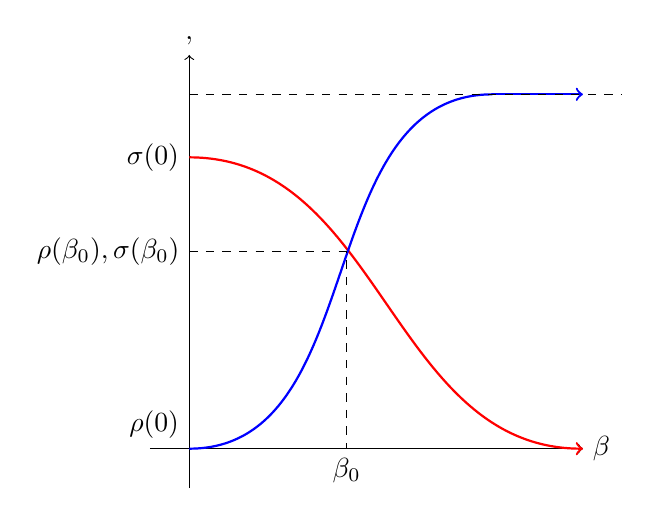
\begin{tikzpicture}[domain=0:5, samples=21,]
\draw[->] (-0.5,0) -- + (5.5,0) node[right] {$\beta$};
\draw[->] (0,-0.5) -- + (0,5.5) node[above] {$\rb,\sib$};

% graph
\draw[thick, draw=red, ->]
(0,3.7) node[left] {$\sigma(0)$} to [out=0,in=180] (5,0);
\draw[thick, draw=blue]
(0,0) node[above left] {$\rho(0)$} to [out=0,in=180] (3.85,4.5);
\draw[thick, draw=blue, ->]
(3.85,4.5) to (5,4.5);
\draw[dashed]   (0,2.5) node[left]  {$\rho(\beta_0),\sigma(\beta_0)$}  -|
            (2, 0)              node[below] {$\beta_0$};
\draw[dashed]   (0,4.5) node[left] {$\za$} to (5.5,4.5);
\end{tikzpicture}
\end{centering} 
%\begin{tikzpicture}[domain=0.5:4.5, samples=17]
%% axes
%\draw[->] (-0.5,0) -- node[below=5mm] {$f$ is decreasing}
%                      + (5.5,0) node[right] {$x$};
%\draw[->] (0,-0.5) -- + (0,5.5) node[above] {$y$};
%% graph
%\draw[line width=2pt, draw=red, ->] 
%    plot (\x,{7-3*sqrt(\x)}) node[right]  {$f(x)$};
%%
%\draw[dashed]   (0,{7-3*sqrt(2)})   node[left] {$f(x_1)$}  -|
%                (2, 0)              node[below] {$x_1$}
%                (0,{7-3*sqrt(3)})   node[left] {$f(x_2)$}  -|
%                (3, 0)              node[below] {$x_2$};
%\end{tikzpicture}
\end{proof}

%%%%%%%%%%%%%%%%%%%%%%%%%%%%%%%%%%%%%%%%
%      MARK LEMMA 6
%%%%%%%%%%%%%%%%%%%%%%%%%%%%%%%%%%%%%%%%
\section{More advanced properties of solutions}
We fix $\beta = \beta_0$. This fixes at least $\nu = \nu_{\beta_0} ~ \text{and}
~ \rho_0 = \rho_{\beta_0}$, which will be used in the following lemma.   
% $\nu = \nu_{\beta_0}$ and $\rho_0 = \rho \left( \beta_0 \right)$. 
We will apply the Sturm comparison theorem to equations \eqref{genwivp} and 
\eqref{nuivp} in the following lemma.

\begin{lemma}\label{genlem6}
For $\alpha\in G\cup N$, $~w(r,\a)$ has a unique zero $r_0\in(0,z(\alpha)).$
Furthermore, \hfill\\ $w(z(\alpha))<0$ for $\a\in N$ and if $\a\in G$, we have
\[
\underset{r\to\infty}{\lim}w(r)=-\infty.
\]
\end{lemma}
\begin{proof}
\revgroup With the simplifications from before, we have
% \be \label{nulivp}
% \nu'' + \frac{1}{r} \nu' + \left[ p V(r) u(r)^{p-1} - \lambda \right] \nu < 0
% \quad \text{and} ~ \nu < 0 \quad \text{on} ~ (0, \rho_0)
% \ee
% 
% whereas
% \be \label{nugivp}
% \nu'' + \frac{1}{r} \nu' + \left[ p V(r) u(r)^{p-1} - \lambda \right] \nu < 0
% \quad \text{and} ~ \nu < 0 \quad \text{on} ~ (\rho_0, \za).
% \ee
% 
\be \label{nulivp} \begin{dcases}
\nu'' + \frac{1}{r} \nu' + \left[ p V(r) u(r)^{p-1} - \lambda \right] \nu < 0
\quad \text{and} ~ \nu > 0 \quad \text{on} ~ (0, \rho_0) \quad \text{and}\\
\nu'' + \frac{1}{r} \nu' + \left[ p V(r) u(r)^{p-1} - \lambda \right] \nu > 0
\quad \text{and} ~ \nu < 0 \quad \text{on} ~ (\rho_0, \za).
\end{dcases} \ee\endgroup

\donegroup Thus $\nu$ has a unique zero $\rho_0$ on $(0, \za)$.  Moreover,
$\nu(0) = \beta_0 \a > 0$ and $\underset{r\to 0}{\lim} ~ r\nu'(r) = 0$. 
%Thus, $\nu(0) > 0$.  
Furthermore, if $\a\in N$, then $\nu(\za) = \za u'(\za) < 0$ by Lemma
\ref{genlem2}. Thus, $\rho_0$ is a unique zero of $\nu$ on  $[0,\za]$.\endgroup

Let $\tau \in (0,\za)$ be the first zero of $w$, which exists by Lemma
\ref{genlem3}. We remember that $w$ satisfies
\be \label{wivp}
w'' + \frac{1}{r} w' + \left[ p V(r) u^{p-1} - \lambda w \right] w = 0
\quad \text{for} ~ r \in (0, \za),
\ee

with initial data $w(0) = 1$ and $\underset{r\to 0}{\lim} rw'(r) = 0$. Because
of this, by \# sturm, we know that $\nu$ oscillates faster than $w$.

Then $\rho_0 \in (0,\tau)$ and thus
\be \label{nutivp}
\nu'' + \frac{1}{r} \nu' + \left[ p V(r) u(r)^{p-1} - \lambda \right] \nu < 0
\quad \text{and} ~ \nu < 0 \quad \text{on} ~ (\tau, \za).
\ee

Since $w(\tau)=0$ and $\nu$ has no zero larger than $\rho_0$, by Sturm we have
that $w$ has no further zero in $(\tau, \za)$ and we can set $r_0 = \tau$. If
$\za < \infty$, then $w$ has no zero on $(\tau, \za]$ and we have $w(\za) < 0$.

However, if $\za = \infty$, we can apply Lemma 6 of \cite[p.~249]{kwong}. The
disconjugacy interal $(d, \infty)$ is such that 
\[ d < \rho_0 < r_0. \]

\donegroup
The disconjugacy interval of a differential equation is the largest
left-neighbourhood $(c, b)$ of the {\red right most} $b$ on which there
exists a solution to the differential equation without zeroes. From Sturmian
theory, no non-trivial solution can have more than one zero in $(c, b)$. On
the other hand, unless $c = a$, with $a$ the {\red left most}, any solution
of the differential equation with a zero before $c$ must have another zero
in $(c, b)$. 
\endgroup

Consider the same setting: equations \eqref{sturm:uivp} and
\eqref{sturm:vivp} satisfying the comparison condition
\eqref{sturm:compare}. In addition, we assume that $U \neq V$ in \emph{any}
neighborhood of $b$. If there exists a solution $V$ of \eqref{sturm:vivp}
with a largest zero at the point $\rho$, then the disconjugacy interval of
\eqref{sturm:uivp} is a strict superset of $(\rho, b)$. 

One way to interpret the above is to remember that $V$ oscillates faster
than $U$ and note that any solution $U$ with a zero in $(\rho, b)$ 

Indeed, if we had $\rho_0 \leq d$, we could find a solution $\tilde{w}$ linearly
independent of $w$ such that $\tilde{w}(\tilde{r}) = 0$ for some $\tilde{r} > d
\geq \rho_0$. But then $w + \tilde{w}$ is a solution of \# $w$ ivp with two
zeroes in $(\rho_0, \infty)$ and thus, $\nu$ should have another zero in {\red that
interval}. By this contradiction, we have $w(r_0) = 0$ with $r_0 \in (d,
\infty)$ and Lemma 6 of \cite[p.~249]{kwong} implies that
\[ \underset{r\to\infty}{\lim} w(r) = -\infty. \]


% Interpreting the statements in this lemma, we will see that $w(r,\a)$ has a
% \textbf{unique} zero $r_0$ to the left of $z(\alpha)$, the zero of the solution
% $u(r,\a)$. When concerned with a ground state solution, $u(r,\a)$ has no finite
% zero, signified by $z(\alpha)=\infty$. Then still $w(r,\a)$ has a finite zero
% $r_0\in(0,\infty)$ and $w(r,\a)<0$ for $r>r_0$ and after $r_0$ the function
% $w(r,\a)$ tends to negative infinity for $r\to\infty$, that is
% $\underset{r\to\infty}{\lim}w(r)=-\infty$.
% 
% Remember that the differential equation in $\nu_{\beta}(r)$ changes sign when
% equal to a value of $\phi_\beta(r)$. In turn, this function $\phi_\beta(r)$
% changes sign in the $r$-value $\sigma(\beta)$. By fixing $\beta=\beta_0$ such
% that $\rho(\beta)$ and $\sigma(\beta)$ intersect in $\beta_0$
% ($\sigma(\beta_0)=\rho(\beta_0)=\rho_0$) we have achieved a crucial step.
% Certain zeroes related to $\nub(r)$ now coincide because of this choice
% $\beta=\beta_0$. Remember that $\phi_{\beta_0}$ changes sign in $r=\rho_0$.
% Which implies that the differential equation in $\nu_{\beta_0}(r)$ changes sign
% in $\rho_0$. But by the definition of $\nub(r)$, we can see that the zero of
% $\nub(r)$ now coincides with the sign change of the differential equation:
% $\rho_0$ is the value in which $\nu_{\beta_0}(r)$ changes sign, since
% $$\nu_{\beta_0}(\rho_0)=-u(\rho_0)\left\{\theta(\rho_0)-\beta_0\right\}=0.$$ The
% last equality follows from $\theta(\rho_0)=\beta_0\iff\rho(\beta_0)=\rho_0$ such
% that $\theta(\rho_0)-\beta_0=0$.
% %
% \begin{gather*}
% \nu''+\frac{1}{r}\nu'+\left[pV(r)u(r)^{p-1}-\lambda\right]\nu<0\quad\text{ on
% }\quad(0,\rho_0)\quad\text{ where }\quad\nu>0\\
% \nu''+\frac{1}{r}\nu'+\left[pV(r)u(r)^{p-1}-\lambda\right]\nu>0\quad\text{ on
% }\quad(\rho_0,\infty)\quad\text{ where }\quad\nu<0 \end{gather*}
% %
% By \# we know that the solution $\nu(r)$ changes sign in
% $\rho_0\in[0,z(\alpha)]$. $$\nu(z(\alpha))z(\alpha)u'(z(\alpha))<0,$$ the
% solution $\nu(r)$ changes sign once. \# expand Since by \# $w(r,\a)$ has at
% least one zero for $\a\in G\cup N$, let $\tau$ be the first zero of $w(r)$. \#
% setup up the Sturm comparison functions for $w$ and $\nu$ and explain Since
% $\nu(r)$ oscillates faster than $w(r,\a)$, there will be a zero to the left of
% $\tau$. That is, $\nu(\rho_0)=0$ with $\rho_0\in(0,\tau)$. 
% 
% Also by Sturm comparison, $w$ can have no further zero and $\tau$ is the unique
% zero of $w$. Suppose that $w$ has a zero with $r_1>r_0$. Then $\nu$ must have a
% zero between $r_0$ and $r_1$. Yet, $\nu$ has a unique zero $\rho_)$, a
% contradiction.
% 
% `'By previous lemmata' the sign of $\nu$ changes in $\rho_0$.  Refer to lemma
% ... and/or figure ...  Also, remember ...  $\nu$ changes sign only once The
% argument that $\nu$ changes sign only once is given in lemma ...  Remember that
% ...  $w$ has a first zero Suppose $w(r)$ does not have a zero.  Then ...
% Comparing $w$ and $v$, conclusion: $w$ has a unique zero One can compare $\nu$
% and $w$ with\\ Sturm's comparison theorem, which is given as ...  In this
% theorem, take ... as ... and ... as ... to see that ...  Also if $\alpha\in G$
% When $\alpha\in G$ then $u(r)$ has no zero.  The solution depends on $\alpha$
% and the change of $u(r)$ with respect to $\alpha$ is given by the function
% $w(r)=\frac{\partial}{\partial\alpha}u(r)$.  `'Since there are solutions that
% have a zero and some that don't', the function $w(r)$ must have a zero.  Even
% more, the zero of $w$ will be to the left of the zero of $u(r)$.
% CIRKELREDENERING?  Then $u(r)$ does not have a zero, the limit of $w(r)$ for $r$
% to infinity is negative infinity.  To see this, note that for increasing
% $\alpha$, one will obtain a solution that \emph{has} a zero.  Hence in that
% $r$-value, the function $u(r)$ decreases with increasing $\alpha$, ergo, the
% function $w(r)$ is increasingly ?? negative for $r$-values where $u(r)$ is
% positive.
\end{proof}

%%%%%%%%%%%%%%%%%%%%%%%%%%%%%%%%%%%%%%%%
%      MARK LEMMA 7
%%%%%%%%%%%%%%%%%%%%%%%%%%%%%%%%%%%%%%%%
\begin{lemma}\label{genlem7}
Let $\a \in G$. There exists $\epsilon > 0$ such that $(\a, \a + \epsilon)
\subset N$. 
\end{lemma}
\begin{proof}
\donegroup
We remember that $w(r)$ has a unique zero $r_0$ by \Cref{genlem6} and since $\a
\in G$, we have $w(r) \to -\infty$ as $r \to \infty$. 
% and $w(r) = w(r, \a) \coloneqq \frac{\partial}{\partial \a} u(r, \a)$. 
This implies by Lemma 6 of \cite[p.~249]{kwong} that $r_0 \in (d, \infty)$,
where $(d, \infty)$ is the disconjugacy interval of initial value problem 
\eqref{genwivp}.  We {\red refer to \#} for the definition of disconjugacy
interval. We can choose $r_1$ and $r_2$
\[ d < r_1 < r_0 < r_2, \]

such that by \eqref{wdef}, there exists $\epsilon > 0$ 
such that for all $\tilde{\a} \in (\a, \a + \epsilon)$, we have
\[
\tilde{u}(r_1) > u(r_1)\quad\text{ and }\quad \tilde{u}(r_2) < u(r_2),
\]
\endgroup
where $\tilde{u}(r) = u(r, \tilde{\a})$. Hence, the graphs of $u$ and $\tilde{u}$
intersect in some $r_3 \in (r_1, r_2)$, where $r_3$ may depend on the choice of
$\tilde{\a}$. Next, we will show that there exists $\tilde{r} \in (r_3, \infty)$
such that $\tilde{u}(\tilde{r}) = 0$. Then, we would have $\tilde{\a} \in N$.

\begin{proof}[Proof step 2.] To see that $\tilde{u}(\tilde{r})=0$ for some
$\tilde{r} \in (r_3, \infty)$, we suppose by contradiction that 
% {\red LATER Hence, $\tilde{\a} \in N$.}
$\tilde{u}(r) > 0$ for all $r > r_3$. We will show that $\tilde{u}(r) < u(r)$
for all $r > r_3$. 
\end{proof}

\begin{proof}[Proof step 3.] To see that $\tilde{u}(r) < u(r)$ for $r > r_3$, we
suppose by contradiction that $\tilde{u}(r_4) = u(r_4)$ for some $r_4 > r_3$ and
$u - \tilde{u} > 0$ on $(r_3, r_4)$.
\end{proof}

The function $z \coloneqq u - \tilde{u}$ satisfies
\be \label{zivp}
z'' + \frac{1}{r} z' + \left[ V(r) \frac{u^p - \tilde{u}^p}{u - \tilde{u}} 
- \lambda \right] z = 0\quad\text{on}~(r_3, r_4). 
\ee

% We shall compare this differential equation with \# w ivp.

Since $z(r_3) = z(r_4) = 0$ by assumption and
\be \label{zcomp} 
\frac{u^p - \tilde{u}^p}{u - \tilde{u}} < pu^{p-1} 
\ee

on $(r_3, r_4)$, we can apply Sturm's theorem \# ref. {\red $w$ oscillates
faster than $z$} Let $y$ be any solution of $w$ ivp linearly independent of
$w$. ... There is no positive solution of $w$ ivp on $(d, \infty)$,
contradicting ...

Hence $z(r) > 0$ for all $r > r_3$. % Then $w$ oscillates faster than $z$.

Sturm comparing fractions

Integrating sturm comparands

Hence $z(r) \equiv u(r) - \tilde{u}(r) \to \infty$ as $r \to \infty$. This is
impossible, since $0 < \tilde{u}(r) < u(r)$ on $(r_3, \infty)$ and $u(r) \to 0$
as $r \to \infty$. Therefore, $\tilde{u}(r)$ must vanish at some point
$\tilde{r} \in (r_3, \infty)$ and the proof is complete.

\end{proof}

%%%%%%%%%%%%%%%%%%%%%%%%%%%%%%%%%%%%%%%%
%      MARK LEMMA 8
%%%%%%%%%%%%%%%%%%%%%%%%%%%%%%%%%%%%%%%%
\begin{lemma}\label{genlem8}
Let $\as \in N$. Then $\left[ \as, \infty \right) \subset N$ and $z : \left[
\as, \infty \right) \to (0, \infty)$ is monotone decreasing.
\end{lemma}
\begin{proof}
$N$ is open subset of $(0, \infty)$ ...

$z$ is continuous ...

By Lemma \ref{genlem6}, we have $w(z(\as)) < 0$. Then, there exists $\epsilon >
0$ such that
\[ (\as, \as + \epsilon) \subset N\quad\text{and}\quad u(z(\as), \a) < 0\quad
\text{for all} ~ \a \in (\as, \as + \epsilon). \]

The intermediate value theorem implies existence of an $r \in (0, z(\as))$ so
that $u(r, \a) = 0$. We note that 
\[ \za \leq r < z(\as)\quad\text{for all} ~ \a \in (\as, \as + \epsilon) \]

and $z$ is decreasing, since ...

We define
\[ \bar{\a} \coloneqq \sup \left\{ \a > \as : \left[ \as, \a \right) \subset N ~
\text{and} ~ z : \left[ \as, \a \right) \to (0, \infty) ~ \text{ is decreasing}
\right\}. \]


By contradiction, we suppose that $\bar{\a} < \infty$. Then there exists ...
\end{proof}

%%%%%%%%%%%%%%%%%%%%%%%%%%%%%%%%%%%%%%%%
%      MARK PROOF
%%%%%%%%%%%%%%%%%%%%%%%%%%%%%%%%%%%%%%%%
\section{Proof of main theorem}
\begin{proof}[Proof of Theorem \ref{genmain}]
\# general proof, referring to lemma's
\end{proof}

\begin{comment}
%%%%%%%%%%%%%%%%%%%%%%%%%%%%%%%%%%%%%%%%
%      MARK OLD MATERIAL
%%%%%%%%%%%%%%%%%%%%%%%%%%%%%%%%%%%%%%%%
\section{Initial value problem and solution sets}
We are interested in the uniqueness of ground state solutions to the soliton
equation \eqref{}. The existence of solutions was treated in chapter \ref{ch2}.
We study the proof by Genoud in \cite{gen11}. Several lemmata will lead to the
conclusion that the set of initial conditions has the following structure
\[ P=(0,\a_0)\quad G=\left\{\a_0\right\}\quad N=(\a_0,\infty) \]

Broadly speaking, we wish to study zeroes of the solution $u(r,\a)$ as a
function of the initial condition $\a$. {\red We define}
\[ \za. \]

By studying the related differential equations in $w(r)$ and $\nu(r)$, and
applying the Sturm comparison theorem, we will show that $z(\a)$ is
monotone decreasing. Furthermore {\red $G$ is open and contiguous}.

Through the chapter, we assume $n=2$. There are more assumptions on $f(u)$
\[ f(u) = \lambda V(r)u(r) - u(r)^p \]

{\red Compare with $f(u)=u-u^3$}.

\section{Lemma 1}
By \# solution set $P$ is non-empty. That is, solutions to \# that are positive
for all $r$ exist. What initial conditions yield such solutions? By studying
the sign of a Lyapunov function $E(r)$ for our problem, we can show that
$(0,\a^*)\subset P$ for certain $\a^*$. \# Expand on Lyapunov. By the initial
value problem, we can show that $E(r)$ is non-increasing for all $r$. This will
separate the initial conditions into $\a\in P$ and $\a\in G\cup N$. After this
lemma, we will study the implications of the latter case.

The Lyapunov (or energy) function can yield information about the solutions.
Let the Lyapunov function be defined as
$$E(r)\coloneqq\frac{1}{2}u'(r)^2-\frac{\lambda}{2}u(r)^2+\frac{1}{p+1}V(r)u(r)^{p+1}$$
on $(0,\za)$. Evaluating the Lyapunov function in $r=0$, we see that the sign
in $r=0$ depends on the initial condition. Solving for $\a$ in
$$E(0)=0\iff-\frac{\lambda}{2}\alpha^2+\frac{1}{p+1}V(0)\alpha^{p+1}=0$$ yields
the critical initial condition
$\a^*=\left[\left(\frac{p+1}{2}\right)\frac{\lambda}{V(0)} \right]^{1/(p-1)}$. 

Additionally, the Lyapunov function $E(r)$ is non-increasing everywhere.
Calculating the derivative as
$$E'(r)=-\frac{u'(r)^2}{r}+\frac{1}{p+1}V'(r)u(r)^{p+1}$$ and using the initial
value problem, we obtain $E'(r)\leq0$ for $r>0$. Now, initial conditions below
$\a^*$ are in solution set $P$. This relies on \#...  

Let $\a\in G\cup N$. The Lyapunov function $E(r)$ evaluated in $r=0$ will now
be greater than or equal to zero. Consider the case for $\a\in N$ and $\a\in G$
seperately. Evaluate the Lyapunov function $E(r)$ in $r=\za$. Clearly,
$E(\za)>0$ \#... Now, evaluate the Lyapunov function $E(r)$ in the limit for
$r\to\infty$. Denote this as \# lim r etc.. $E(\infty)$. Clearly $E(\infty)=0$.
\# weave in ... To see this, note that both $u(r)$ and $u'(r)$ vanish for
$r\to\infty$ and calculate the limit $\underset{r\to\infty}{\lim}E(r)=0$. But
$E(r)$ is non-increasing, so $E(0)\geq0$.

In conclusion, the Lyapunov function $E(r)$ defined for $r>0$ splits the
initial conditions around $\a^*$. That is, $\a_P<\a^*<\a_{G\cup N}$. By the
derivative $E'(r)$ and the initial value problem \#, we know that $E(r)$ is
non-increasing for $r>0$. Lastly, for $\a\in P$ we have $E(0)<0$. And for
$\a\in G$ we have $E(0)\geq0$ and for $\a\in N$, we have $E(0)>0$.

Note: \# Similarly, for $\a\in N$, the solution $u(r)$ vanishes in some $\za$.
Evaluating $\underset{r\to\za}{\lim}E(r)=\frac{1}{2}u'(\za)^2$ and noting that
by definition of $N$ we have $u'(\za)\neq0$, we find that $E(0)\geq0$.

Note: \# This begs the question, is $E(0)$ non-negative for all initial
conditions? Solving $E(0)<0$ yields initial conditions that must belong to $P$,
not to contradict the results that for $\a\in G\cup N$ we have $E(0)\geq0$.

This lemma states an interval of initial conditions $0<\a<\ldots$ for which the
corresponding  solution belongs to solution set $P$. The proof of the lemma
involves a Lyapunov (or energy) functions $E(r)$ and its derivative $E'(r)$,
which are related to \# the IVP. Enough is known about the terms in the
derivative $E'(r)$ to conclude that the function $E(r)$ is non-increasing for
all $r$. For initial conditions in solution sets $G$ or $N$, the defining
properties of $u(r)$ and $u'(r)$ yield that $E(0)\geq0$. Furthermore, the
function $E(r)$ is non-increasing, so that for any $r\geq0$ we have
$E(r)\geq0$. This splits the initial conditions in two sets, as we will see,
for $\a\in G\cup N$ we have $E(0)\geq0$. Suppose that there are initial
conditions which have $E(0)<0$, the the assumption that these belong to $G$ or
$N$ leads to a contradiction since that would imply $E(0)\geq0$. Then these
initial conditions must belong to solution set $P$. The actual upper bound in
$0<\a<\ldots$ arises from solving $E(0)<0$.

\begin{proof}
Define the Lyapunov (or energy) function $E(r)$ on $(0,\za)$ as:
$$E(r)\coloneqq\frac{1}{2}u'(r)^2
-\frac{\lambda}{2}u(r)^2+\frac{1}{p+1}V(r)u(r)^{p+1},$$
We directly calculate the derivative $E'(r)$ and use the \cref{ivp} to simplify. 
\begin{align*}
&\left[u''(r)-\lambda u(r)+V(r)u(r)^p\right]=
-\frac{1}{r}u'(r)\quad\text{from the IVP, and}\\
E'(r)&=u''(r)u'(r)-\lambda u(r)u'(r)+V(r)u(r)^pu'(r)+\frac{1}{p+1}V'(r)u(r)^{p+1}\\
&=\left[u''(r)-\lambda u(r)+V(r)u(r)^p\right]u'(r)+\frac{1}{p+1}V'(r)u(r)^{p+1}\\
&=-\frac{u'(r)^2}{r}+\frac{1}{p+1}V'(r)u(r)^{p+1}\leq0\text{ for }r>0.\\
\end{align*}
We know that $E'(r)$ is non-positive for $r>0$, because:
\begin{easylist}[itemize]
@ $V'(r)\leq0$, by hypothesis H2;
@ $u(r)^{p+1}\geq0$ because $u(r)$ is positive on $(0,z(\a))$ for any initial condition $\a$;
@ $r\geq0$;
@ $u'(r)^2\geq0$.
\end{easylist}
Then $E(r)$ is non-increasing $(0,z(\a))$.

Suppose $\a\in G$. Then $u(r)\to0$ and $u'(r)\to0$ as $r\to\infty$. Then $E(r)=0$ for $r\to\infty$. In conclusion $E(0)\geq0$.
Alternatively, suppose $\a\in N$, then $u(\za)=0$. Now evaluate:
\begin{empheq}{align*}
\underset{r\to z(\alpha)}{\lim}E(r)&=\underset{r\to z(\alpha)}{\lim}\bigg[\frac{1}{2}u'(r)^2-\frac{\lambda}{2}u(r)^2+\frac{1}{p+1}V(r)u(r)^{p+1}\bigg] \\
&=u'(z(\alpha))^2\geq0.
\end{empheq}
As $E(r)$ is non-increasing, $E(0)\geq0$.
Result: $E(0)\geq0$ and $E(r)$ well-defined on $[0,z(\a)]$ for $\a\in G\cup N$.

\emph{Proof step} We solve $E(0)=0$ to find an upper bound $0<\a<\ldots$ such that $E(0)<0)$:
\begin{align*}
E(0)=~&\frac{1}{2}u'(0)^2-\frac{\lambda}{2}u(0)^2+\frac{1}{p+1}V(0)u(0)^{p+1}<0\\
&\iff -\frac{\lambda}{2}\alpha^2+\frac{1}{p+1}V(0)\alpha^{p+1}<0\\
&\iff\alpha^{p-1}<\left(\frac{p+1}{2}\right)\frac{\lambda}{V(0)}\\
&\iff\alpha<\left[\left(\frac{p+1}{2}\right)\frac{\lambda}{V(0)} \right]^{1/(p-1)}
%
% \iff\alpha^{p-1}<\left(\frac{p+1}{2}\right)\frac{\lambda}{V(0)}\iff
%\frac{1}{p+1}V(0)\alpha^{p-1}<\frac{\lambda}{2}\\
% -\frac{\lambda}{2}\alpha^2+\frac{1}{p+1}V(0)\alpha^{p+1}<0\\
% \implies E(0)=\frac{1}{2}u'(0)^2-\frac{\lambda}{2}u(0)^2+\frac{1}{p+1}V(0)u(0)^{p+1}<0.
\end{align*}
In conclusion, we have $\a\in P$ whenever $0<\a<\left[\left(\frac{p+1}{2}\right)\frac{\lambda}{V(0)}\right]^{1/(p-1)}$.
\end{proof}




\section{Lemma 2}
To separate the solutions corrsponding to initial conditions belonging to $G$ or $N$, we need to study the zero (or zeroes) of $u(r,\a)$. This can not be done directly. However, it can be shown directly that all solutions with initial condition in $G$ or $N$ are decreasing everywhere. That is, $u'(r,\a)<0$ where the derivative is with respect to $r$. 

%Goal: This lemma aims to show that the solution decreases everywhere on $(0,\za)$ for $\a\in G\cup N$ and for $\a\in N$ even $u'(\za)<0$. This is an important step in showing that $w(r)$ has a unique zero on $(0,\za)$, which is the central step to showing that $\a\in G$ is unique.

This will be done again by studying the Lyapunov function $E(r)$. Note that the assumption "$V(0)$ is finite" is no longer present. From the previous lemma and the IVP it follows, in either case, that $u''(0)<0$ and $u'(0^+)<0$. If $V(0)$ is finite, then \#. If $V(0)$ is infinite, then \#. 

Suppose now that the derivative of the solution with respect to $r$ vanishes in $r_0$, that is $u'(r_0)=0$ for some $r_0$. Then the \cref{ivp} yields an equation in $u(r_0)$ and $u''(r_0)$. By concavity of the graph of the solution $u(r)$, we have $u''(r_0)>0$. Expand concavity argument \#. Then using the Lyapunov function evaluated in $r_0$, we find $E(r_0)<0$ which contradicts the assumption that $\a\in G\cup N$. Give evaluation \#. Hence, $u'(r)<0$ everywhere.

In conclusion, the solution sets $G$ and $N$ have $u'(r)<0$ everywhere on $(0,\za)$ for $\a\in G$ and $(0,\za]$ for $\a\in N$. The lemma shows $u(r)$ strictly decreasing on $(0,\za)$ for $\a\in G\cup N$. The rest of the proof uses this to conclude that $w(r)$ has a unique zero on $(0,\za)$. Finally, analysis of solution sets $N$ and $G$ leads to the uniqueness result. Write $\za=\infty$ when $\a\in G$, since $u(r,\a)\to0$ as $r\to\infty$. Let $\a\in G\cup N$. By lemma \# 4 (1?), $E(r)\geq0$ on $[0,\za]$ and non-increasing.

Question: what is an example of infinite $V(0)$ and is it relevant for my thesis? Problem with $E(0)=...V(0)$, might blow up.

\begin{proof}
By \cref{ivp}, we have $E(r)\geq0$ in the limit that $r$ goes to $\za$. Since $E(r)$ is non-increasing, $E(r)\geq0$ for all $r\in(0,\za]$. Note that $E(0)$ is no longer well-defined as the assumption that $V(0)$ is finite is no longer present.

\# Lemma 1 and the \# \cref{ivp} yield $u''(0)<0$ and $u'(r)<0$ for $r>0$ and small. No explicit argument is presented in \# Genoud. The argument that $u''(0)<0$ is not expanded upon here. To see why $u''(0)<0$ implies $u'(r)<0$ for $r>0$ and small, reason by concavity. Since $u''(0)<0$, the graph is concave down. This implies that $u'(r)<u'(0)$ for $r>0$ and small. 

This result $u'(r)<0$ for $r$ small, can be extended for larger $r$, even up to (or including) $\za$. Suppose by contradiction that $r_0=\inf(r<\za,u'(r)=0)$ exists. That is, the derivative $u'(r)$ vanishes in $r_0$ or $u'(r_0)=0$. This implies that $u''(r)$ was positive on $(r,r_0)$ for some $r>0$. Both $u''(r_0)=0$ and $u''(r_0)>0$ lead to a contradiction. The combination of $u''(r_0)$ and $u'(r_0)=0$ would imply $u\equiv u(r_0)$, a contradiction. To see how $u''(r_0)>0$ leads to a contradiction, invoke the \# \cref{ivp}: 
\begin{align*}
&u''(r_0)=\lambda u(r_0)-V(r_0)u(r_0)^p>0\\
\implies &u(r_0)<\left[\frac{\lambda}{V(r_0)}\right]^{1/(p-1)}<\left[\left(\frac{p+1}{2}\right)\frac{\lambda}{V(r_0)}\right]^{1/(p-1)}\\
\text{\# suppose that }u(r_0)\neq0\\
\iff &u(r_0)<\left[\frac{\lambda}{V(r_0)}\right]<\left[\left(\frac{p+1}{2}\right)\frac{\lambda}{V(r_0)}\right]^{1/(p-1)}\\
\text{since }\frac{p+1}{2}>1\\
\iff &u(r_0)^{p-1}<\left(\frac{p+1}{2}\right)\frac{\lambda}{V(r_0)}\\
\iff &\frac{1}{p+1}V(r_0)u(r_0)^{p+1}<\frac{\lambda}{2}u(r_0)^2\\
\iff &-\frac{\lambda}{2}u(r_0)^2+\frac{1}{p+1}V(r_0)u(r_0)^{p+1}<0
% \implies E(r_0)=-\frac{\lambda}{2}u(r_0)^2+\frac{1}{p+1}V(r_0)u(r_0)^{p+1}<0,
\end{align*}
Then evaluating the Lyapunov function $E(r)$ with the assumption $u'(r_0)=0$, this yields $E(r_0)<0$:
$$ E(r_0)=-\frac{\lambda}{2}u(r_0)^2+\frac{1}{p+1}V(r_0)u(r_0)^{p+1}<0 $$
But $E(r_0)<0$ contradicts $E(r)\geq0$, so $u'<0$ on $(0,z(\alpha))$.

To see that $u'(\za)<0$ when $\a\in N$, suppose by contradiction that $u'(\za)=0$ and remember that by definition $u(\za)=0$. Then $u\equiv0$, because by the \# \cref{ivp} we have that $u''(\za)=\lambda u(\za)-V(\za)u(\za)^p=0$. \# Contradiction: the solution $u=\equiv$ is not in $N$.

\underline{Conclusion:} $u'(z(\alpha))<0$ for $r\in(0,\za)$ if $\a\in G$ and $r\in(0,\za]$ if $\a\in N$.
\end{proof}



\section{Lemma 3}
Even though solutions in sets $G$ and $N$ have been shown to be decreasing everywhere, there is no information about the zeroes. In this lemma, through the Lagrange identity, information about zeroes of the derivative of the solution with respect to the initial condition can be achieved. Define $$w(r,\a) = \frac{\partial}{\partial\a} u(r,\a)$$ and evaluate the Lagrange identity for \# and \# in $0$ and $\za$. The conclusion will be that $w(r,\a)$ changes sign at least once on $(0,\za)$. Later, this result will be improved, the zero of $w(r,\a)$ is unique and this ultimately leads to the uniqueness of the ground state solution. But for now, enough work to do!

\begin{proof}
The Lagrange identity for \cref{ivp} and \cref{wvp} will yield information about the zeroes of $w(r)$. The cases $\a\in N$ and $\a\in G$ will be considered seperately. First, suppose $\a\in N$. The differential equations for $u$ and $w$ can be written as:
\begin{gather*}
(ru'(r))'+r\left[-\lambda u(r)+V(r)u(r)^p\right]=0\\
(rw'(r))'+r\left[-\lambda w(r)+pV(r)u(r)^{p-1}w(r)\right]=0.
\end{gather*}
Multiply these equations by $w(r)$ and $u(r)$ respectively and subtract to obtain:
\begin{gather*}
z(\alpha)w(r)(ru'(r))'-u(r)(rw'(r))'=r\left\{pV(r)u(r)^pw(r)-V(r)u(r)^pw(r)\right\},
\end{gather*}
Now integrate from $0$ to $\za$ to obtain: 
\begin{gather*}
\int_0^{z(\alpha)}w(r)(ru'(r))'-u(r)(rw'(r))'dr=
\int_0^{z(\alpha)}r\left\{pV(r)u(r)^pw(r)-V(r)u(r)^pw(r)\right\}dr.
\end{gather*}
Now perform partial integration for the left hand side and remember $u(z(\a))=0$:
% \begin{align*}
%   rw(r)u'(r)\at_0^{z(\alpha)}-ru(r)w'(r)\at_0^{z(\alpha)}&-
%   \int_0^{z(\alpha)}\underbrace{\{ru'(r)w'(r)-ru'(r)w'(r)\}}_0dr\\
%   &=(p-1)\int_0^{z(\alpha)}rV(r)u(r)^pw(r)dr\\
%   z(\alpha)w(z(\alpha))u'(z(\alpha))&=(p-1)\int_0^{z(\alpha)}rV(r)u(r)^pw(r)dr.
% \end{align*}

For $\a\in N$, note $r>0,~V>0,~u^p>0$ are finite almost everywhere. Suppose $w>0$ on $(0,z(\alpha))$. Then the left hand side and right hand side disagree, $$z(\alpha)u'(z(\alpha))w(z(\alpha))<0\text{, while }(p-1)\int_0^{z(\alpha)}rV(r)u(r)^pw(r)dr>0.$$ A similar argument holds for $w<0$. \underline{Conclusion:} $w$ changes sign at least once on $(0,z(\a))$.

For $\alpha\in G$, suppose by contradiction that $w>0$ on $(0,\infty)$.
Integrate \# \cref{ivp} from $0$ to $r$ and rewrite the left hand side using the quotient rule:
\begin{align*}
ru'(r)w(r)-rw'(r)u(r)
=r\frac{u'(r)w(r)-w'(r)u(r)}{w(r)^2}
&=rw(r)^2\left(\frac{u(r)}{w(r)}\right)'\\
rw(r)^2\left(\frac{u(r)}{w(r)}\right)'
&=(p-1)\int_0^{z(\alpha)}rV(r)u(r)^pw(r)dr>0.
\end{align*}
By similar reasoning as before, the right hand side is still positive. Hence, the left hand side is also positive. This implies that the term quotient of $u$ and $w$ is increasing.
\underline{Result:} $\left(\frac{u}{w}\right)'$ is positive, so $\frac{u}{w}(r)$ is increasing.

Before, the left hand side was contradictory by simple reasons. Unfortunately, this is not the case now. In summary,  by Lemma C.1 of \cite{fthes}, for $\a>0$ the quantity $\frac{u(r)}{w(r)}$ vanishes in the limit that $r\to\infty$. This contradicts the earlier assumption that $\frac{u}{w}(r)$ is increasing.
\# Is it really this simple? What about Theoreme 1.4.9. And the subtlety in having asymptotic behaviour of both w and u?

In conclusion, for $\a\in G$ the assumption that $w>0$ is again contradictory. \# and for $w<0$... Hence, $w$ changes sign at least once on $(0,z(\a))$ for $\a\in G\cup N$.
\end{proof}

\section{Lemmata A}
The previous result can be improved upon. In fact, $w$ can be shown to have a unique zero. With the Sturm comparison theorem, this can be used to construct more lemmata and finally to show that $G$ contains at most one element, i.e. the ground state solution is unique.

In the lemmata following, many related properties are used. This section is dedicated to properly introducing those functions and their properties. A \emph{shopping list}: we will introduce $\theta(r)$, $\rho(\beta)$, $\nu_\beta(r)$, $\phi_\beta(r)$. Then lemma 4 introduces $\sigma(\beta)$, $\xi(r)$, $\Xi(r)$. All of these functions are related to the original initial value problem in $u(r)$, to the problem in $w(r)$ or to the problem $\nu(r)$ which is a transformation of the problem in $u(r)$ including the $\beta$ parameter. This $\beta$ will be fixed in lemma 5 to construct a zero $\rho_0$ for the $\nu(r)$ problem. In lemma 6 the problem in $\nu(r)$ and $w(r)$ are Sturm compared to show that the zero of $w(r)$ is unique. The uniqueness of the zero of $w(r)$ will translate to the monotone decreasing $\za$ which translates to the structure of $I=P\cup G\cup N$ and the required uniqueness result.

First, define the function $\theta(r)$ as: 
$$\theta(r)\coloneqq-r\frac{u'(r)}{u(r)}\text{, for }r\in[0,z(\alpha).$$ 
The limit for $r$ to zero is calculated as: 
$$\theta(0)=\underset{r\downarrow0}{\lim}\theta(r)=\underset{r\downarrow0}{\lim}\left(-r\frac{u'(r)}{u(r)}\right)=\underset{r\downarrow0}{\lim}\frac{-ru'(r)}{\a}=0.$$ 
Combined with the fact that $\theta(r)$ is increasing ($\theta'(r)>0$), we have $\theta(r)>0$ on $(0,\za)$, \# argument that $\theta$ is increasing. 
Lastly, the function is unbounded as $\underset{r\to\za}{\lim}\theta(r)=\infty$. To see this, let $\a\in N$ then $\za$ is the first zero of the solution $u(r,\a)$. Also, by \# the derivative is negative everywhere. Hence by definition of $\theta(r)$ the limit for $r\to\za$ is infinity. A similar argument holds for $\a\in G$.

The function $\theta(r)$ is continuous and increasing, so there exists an
inverse function. We define $\rho \coloneqq \theta^{-1}$. Then
\[
\rb = r \iff \theta(r) = \beta.
\]

But what are the properties of this inverse function $\rb$? First, we must have
$\rho(0) = 0$ and $\underset{\beta\to\infty}{\lim} \rb = \za$. Note how $\rb$
too is continuous and increasing, but with respect to $\beta$. Note that $\rb$
is positive, that is, $\rb > 0$ on $(0, \infty)$. \# image of $\theta(r)$ and
inverse $\rb$. 

Now define a transformed version of the \# $$\nu_{\beta}(r)\coloneqq ru'(r)+\beta u(r)=-u(r){\theta(r)-\beta}.$$ 
While the solution $u(r,\a)$ was positive everywhere on $(0,\za)$ this is not necessarily true for $\nub$. 
Note that $u(r)>0$ so $\nub>0$ if $\tr-\beta<0$. 
That is, $0>\tr-\beta\iff\beta>\tr\iff\rb>r$. 
Let $\beta>0,$ then $\nu_{\beta}(r)>0$ if $r<\rho(\beta)$ and $\nu_{\beta}(r)<0$ if $r>\rho(\beta)$. 
Similarly, $\nub<0$ if $\beta<\tr\iff\rb<r$. 
All of these properties can also be illustrated \#. 

To see that $\nu_{\beta}(r)$ satisfies the differential equation... 
$$\nu_{\beta}''(r)+\frac{1}{r}\nu_{\beta}(r)'-\lambda\nu_{\beta}+pV(r)u(r)^{p-1}\nu_{\beta}=\phi_{\beta}(r)$$
where the function $\phib(r)$ on the right hand side is defined as $$\phi_{\beta}(r)\coloneqq\left[\beta(p-1)-2\right]V(r)u(r)^p-rV'(r)u(r)^p+2\lambda u(r).$$
\# derivation must be somewhere

In lemma 4 the above w \# argument will be used to show that the sign of $\phib(r)$ is related to a continuous decreasing function $\sib(r)$ and this function intersects $\rb$ in a unique $\beta_0$ (lemma 5). The specific $\nu_{\beta_0}$ and $\rho_0=\rho(\beta_0)$ are used in lemma 6 with the Sturm comparison theorem to show that $w$ has a unique zero on $(0,\za)$.


\section{Lemma 4}
\begin{proof}
Why is this $\sigma$ unique? Maybe because inverse of uniquely defined $\rb$?
There are infinitely many functions that agree with $\sigma(0)>0$ and $\sigma(\bar{\beta})=0$. Clearly, the other property of $\sigma$ uniquely defines the function. 
Let $\beta$ be arbitrary. This makes $\phib(r)$ fixed. 
\# Argument why $\phib$ changes sign only once. 
Then $\sib$ is defined by the zero of $\phib$. 
Since $\beta$ was arbitrary, $\sib$ is defined by $\phib$ for all $\beta$ and $\sib$ is unique. 
That $\sib$ is continuous and decreasing is shown below.

%Draw the following: $x$-axis is the $\beta$-axis and goes from 0 to $\bar{\beta}$. The $y$-axis is the $r$-axis and goes from 0 (in $\bar{\beta}$) to some finite number $\sigma(0)>0$. For any $\beta$ between 0 and $\bar{\beta}$ there is a corresponding $\sigma(\beta)$. As this value needs to agree with the property of $\phi_{\beta}(r)$--$\phi_{\beta}(r)<0$ for $r<\sigma(\beta)$ and $\phi_{\beta}(r)>0$ for $r>\sigma{\beta}$-- for all $\beta$ then $\sigma$ is uniquely defined!
To analyse the function $\phib(r)$ we will write the function more conveniently. We know that $r>0$ and $V(r)>0$ and $u(r)^p>0$ and this will allow us to assert the sign of a part of the function $\phib(r)$. In $\phib(r)$, factor out a term of $V(r)u(r)^p>0$ and gather the other terms into $\xi(r)$ as follows:
\begin{align*}
\phi_{\beta}(r)&=\left[\beta(p-1)-2\right]V(r)u(r)^p-rV'(r)u(r)^p+2\lambda u(r) \\ %\\ &=V(r)u(r)^p\left[\beta(p-1)-2-\frac{rV'(r)u(r)^p}{V(r)u(r)^p}+\frac{2\lambda u(r)}{V(r)u(r)^p}\right]\\ 
&=V(r)u(r)^p\left[\beta(p-1)-2-r\frac{V'(r)}{V(r)}+\frac{2\lambda}{V(r)u(r)^{p-1}}\right]\\ 
&= V(r)u(r)^p\left[\beta(p-1)-2-\xi(r)\right]\\
\text{where }\xi(r)&=r\frac{V'(r)}{V(r)}-\frac{2\lambda}{V(r)u(r)^{p-1}}.
\end{align*}
% Now, let $\beta>0$ arbitrarily and let $r\in[0,z(\alpha))$. 

Hence the sign of $\phi(r)$ depends on $\beta$ and $\xi(r)$ by the term in brackets. Remember that $p$ is just a constant of the initial value problem resembling a dimension \#. Note that $\phib(r)>0 \iff \left[\ldots\right]>0$. This allows us to solve for $\beta$:
$$\beta(p-1)-2-\xi(r)>0\iff\beta>\frac{2+\xi(r)}{p-1}\coloneqq\Xi(r).$$
That is, $\phib(r)$ is positive whenever $\beta$ is greater than this new function $\Xi(r)$. Studying this function $\Xi(r)$ will be our next step.

Before studying the sign of and bounds on $\Xi(r)$, we can show that the function $\xi(r)$ is non-positive and strictly decreasing on the usual interval.. In other words: $$\xi(r)\leq0\text{ and }\xi'(r)<0\text{ on }(0,\za).$$ This implies that the limit approaches negative infinity: $$\lim_{r\to z(\alpha)}\xi(r)=-\infty.$$ To see this, note how the first fraction in the expression for $\xi(r)$ is nonincreasing: $$h(r)=r\frac{V'(r)}{V(r)}$$ as the numerator $V'(r)$ is negative everywhere, the denominator $V(r)$ is positive everywhere and of course $r>0$. By similar reasoning, the second term of $\xi(r)$ is strictly decreasing. We know that $V(r)$ is decreasing and so is $u(r)$ (hence $u(r)^{p-1}$ as well). Since the numerator $\lambda>0$ is constant and the denominator is strictly decreasing, the fraction is strictly increasing such that the second term of $\xi(r)$ is strictly decreasing. Thus $\xi(r)$ is strictly decreasing. Since $u(z(\alpha))=0$, the limit is $-\infty$. Even if $V(r)$ is non-zero, then still, the fraction blows up by the behaviour of $u(r)$ near $\za$.

Next, we can show that $\Xi(0)>0$ and $\Xi(r)$ is continuous and strictly decreasing. First $\Xi(r)$ is strictly decreasing because $\xi(r)$ is strictly decreasing and $\Xi(r)$ is a monotonous transformation \# ?. By similar argument, $\Xi(r)$ is continous. $\Xi(r)=\left[2+\xi(r)\right]/(p-1)$ satisfies $\Xi(0)>0$. To see that $\Xi(0)>0$, evaluate $\xi(r)$ in $r=0$ and compare: $$\Xi(0)>0\iff\xi(0)>-2.$$

Evaluating $\xi(0)$ for infinite $V(0)$ relies on \#. When $V(0)=\infty$ then the second term in $\xi(0)$ is zero, since $u(0,\a)^{p-1}=\a^{p-1}$. Then $\xi(0)=h_0$. And by \# $h_0+k\geq0$ so $h_0>-k$. Since $k\in(0,2)$ the lowest bound for $h_0$ is $-k>-2$. Alternatively, when $V(0)$ is finite, then $h_0=0$ by \#. Then $$\xi(0)=-\frac{2\lambda}{\a^{p-1}V(0)}.$$ Now we can solve for $\a$ to find the values of $\a$ for which $\xi(0)>-2$.
\begin{align*}
-\frac{2\lambda}{\a^{p-1}V(0)}>-2\\
\frac{\lambda}{\a^{p-1}V(0)}<1\\
\frac{\lambda}{V(0)}<\a^{p-1}\\
\a > \left[\frac{\lambda}{V(0)}\right]^{\frac{1}{p-1}}
\end{align*}
which is confirmed by the assumption that $\a\in G\cup N$ \# is it?.

Trailing back our steps, we see that $\xi(0)>-2$ which implies $\Xi(0)>0$. For any $\beta\in(0,\bar{\beta})$ we have $$\beta<\Xi(r)\iff\beta(p-1)-2-\xi(r)<0\quad\text{ and vice versa.}$$ 

\# conclude that this verifies the existence of the unique function $\sigma(\beta)$ with the aforementioned properties. that is $\sigma(\beta)$ is continuous and decreasing and $\sigma(0)>0$ and $\sigma(\bar{\beta})=0$ as well as $\sigma(\beta)$ determing the sign of $\phi_\beta(r)$ for all $\beta>0$.

% Now that we have confirmed $\Xi(0)>0$ and $\Xi(r)$ strictly decreasing... \# Let $\Xi(0)=\bar\beta$, \#, for all $\beta\in[0,\bar\beta]$. Note $\Xi(r)$ is continuous and decreasing, so $\sigma(\beta)\coloneqq\left.\Xi(r)^{-1}\right|_{[0,\bar\beta]}$ has properties (a) and (b).\# Also, note $\Xi(0)>0\iff\xi(0)>-2$. \# \# 
% Show that there is an implication from the property of $V(0)$ to the property of $\xi(0)$. By definition? $\xi(0) = 0 * V'(0)/V(0) + 2\lambda / (V(0)*u(0)^{p-1}$... What do I know about $V'(0)?$ And about $V(0)?$ By lemma 5.1 ?? 
% % % % % % % % Also, as $u(0,\a)=\a>0$, we have $\a^{p-1}>0$ and $V(0)>0$ (finite or infinite) implies the second term of $\xi > 0$... Yes, definitely some Lyapunov/lemma 5.1 property involved here. Consider the following cases ......$V(0)<\infty$ .... $V(0)=\infty$ ... hence $\xi(0)>-2$ for $\alpha\in(G\cup N)$.

\end{proof}
\clearpage
\section{Lemma 5}
\begin{lemma}
Let $\alpha\in G\cup N$.
There exists a unique $\beta_0>0$ such that $\rho(\beta_0)=\sigma(\beta_0)$.
This follows immediately from the aforementioned properties of $\rho(\beta)$ and
$\sigma(\beta)$. Sketching the two graphs, there is a unique
intersection.\hfill\\

\begin{centering}
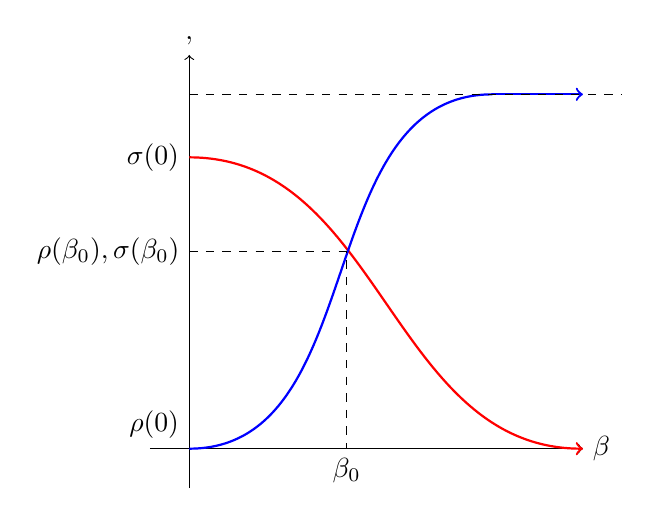
\begin{tikzpicture}[domain=0:5, samples=21,]
\draw[->] (-0.5,0) -- + (5.5,0) node[right] {$\beta$};
\draw[->] (0,-0.5) -- + (0,5.5) node[above] {$\rb,\sib$};

% graph
\draw[thick, draw=red, ->]
(0,3.7) node[left] {$\sigma(0)$} to [out=0,in=180] (5,0);
\draw[thick, draw=blue]
(0,0) node[above left] {$\rho(0)$} to [out=0,in=180] (3.85,4.5);
\draw[thick, draw=blue, ->]
(3.85,4.5) to (5,4.5);
\draw[dashed]   (0,2.5) node[left]  {$\rho(\beta_0),\sigma(\beta_0)$}  -|
            (2, 0)              node[below] {$\beta_0$};
\draw[dashed]   (0,4.5) node[left] {$\za$} to (5.5,4.5);
\end{tikzpicture}
\end{centering} 
%\begin{tikzpicture}[domain=0.5:4.5, samples=17]
%% axes
%\draw[->] (-0.5,0) -- node[below=5mm] {$f$ is decreasing}
%                      + (5.5,0) node[right] {$x$};
%\draw[->] (0,-0.5) -- + (0,5.5) node[above] {$y$};
%% graph
%\draw[line width=2pt, draw=red, ->] 
%    plot (\x,{7-3*sqrt(\x)}) node[right]  {$f(x)$};
%%
%\draw[dashed]   (0,{7-3*sqrt(2)})   node[left] {$f(x_1)$}  -|
%                (2, 0)              node[below] {$x_1$}
%                (0,{7-3*sqrt(3)})   node[left] {$f(x_2)$}  -|
%                (3, 0)              node[below] {$x_2$};
%\end{tikzpicture}
\end{lemma}



\section{Lemma 6}
%%%%%%%%%%%%%%%%%%%%%%%%%%%%%%%%%
%%%.     CHAPTER 5.6
%%%%%%%%%%%%%%%%%%%%%%%%%%%%%%%%%
\begin{lemma}\label{wq}
For $\alpha\in G\cup N$ the derivative of the solution with respect to the initial condition $w(r,\a)$ has a unique zero $r_0\in(0,z(\alpha)).$ Furthermore, 
\begin{align*}
w(z(\alpha))<0,\quad&\text{ if }\alpha\in N\\
\underset{r\to\infty}{\lim}w(r)=-\infty,\quad&\text{ if }\alpha\in G.
\end{align*}

\begin{proof}
% Some remarks: the functions $u(r)$ and $w(r)$ will be compared `'in the rest of the uniqueness proof'. 
Interpreting the statements in this lemma, we will see that $w(r,\a)$ has a \textbf{unique} zero $r_0$ to the left of $z(\alpha)$, the zero of the solution $u(r,\a)$. When concerned with a ground state solution, $u(r,\a)$ has no finite zero, signified by $z(\alpha)=\infty$. Then still $w(r,\a)$ has a finite zero $r_0\in(0,\infty)$ and $w(r,\a)<0$ for $r>r_0$ and after $r_0$ the function $w(r,\a)$ tends to negative infinity for $r\to\infty$, that is $\underset{r\to\infty}{\lim}w(r)=-\infty$.

Remember that the differential equation in $\nu_{\beta}(r)$ changes sign when equal to a value of $\phi_\beta(r)$. In turn, this function $\phi_\beta(r)$ changes sign in the $r$-value $\sigma(\beta)$. By fixing $\beta=\beta_0$ such that $\rho(\beta)$ and $\sigma(\beta)$ intersect in $\beta_0$ ($\sigma(\beta_0)=\rho(\beta_0)=\rho_0$) we have achieved a crucial step. Certain zeroes related to $\nub(r)$ now coincide because of this choice $\beta=\beta_0$. Remember that $\phi_{\beta_0}$ changes sign in $r=\rho_0$. Which implies that the differential equation in $\nu_{\beta_0}(r)$ changes sign in $\rho_0$. But by the definition of $\nub(r)$, we can see that the zero of $\nub(r)$ now coincides with the sign change of the differential equation: $\rho_0$ is the value in which $\nu_{\beta_0}(r)$ changes sign, since $$\nu_{\beta_0}(\rho_0)=-u(\rho_0)\left\{\theta(\rho_0)-\beta_0\right\}=0.$$ The last equality follows from $\theta(\rho_0)=\beta_0\iff\rho(\beta_0)=\rho_0$ such that $\theta(\rho_0)-\beta_0=0$.
%
\begin{gather*}
\nu''+\frac{1}{r}\nu'+\left[pV(r)u(r)^{p-1}-\lambda\right]\nu<0\quad\text{ on }\quad(0,\rho_0)\quad\text{ where }\quad\nu>0\\
\nu''+\frac{1}{r}\nu'+\left[pV(r)u(r)^{p-1}-\lambda\right]\nu>0\quad\text{ on }\quad(\rho_0,\infty)\quad\text{ where }\quad\nu<0
\end{gather*}
%
By \# we know that the solution $\nu(r)$ changes sign in $\rho_0\in[0,z(\alpha)]$. $$\nu(z(\alpha))z(\alpha)u'(z(\alpha))<0,$$ the solution $\nu(r)$ changes sign once. \# expand Since by \# $w(r,\a)$ has at least one zero for $\a\in G\cup N$, let $\tau$ be the first zero of $w(r)$. \# setup up the Sturm comparison functions for $w$ and $\nu$ and explain Since $\nu(r)$ oscillates faster than $w(r,\a)$, there will be a zero to the left of $\tau$. That is, $\nu(\rho_0)=0$ with $\rho_0\in(0,\tau)$. 

Also by Sturm comparison, $w$ can have no further zero and $\tau$ is the unique zero of $w$. Suppose that $w$ has a zero with $r_1>r_0$. Then $\nu$ must have a zero between $r_0$ and $r_1$. Yet, $\nu$ has a unique zero $\rho_)$, a contradiction.

`'By previous lemmata' the sign of $\nu$ changes in $\rho_0$.
Refer to lemma ... and/or figure ...
Also, remember ...
$\nu$ changes sign only once
The argument that $\nu$ changes sign only once is given in lemma ...
Remember that ...
$w$ has a first zero
Suppose $w(r)$ does not have a zero.
Then ...
Comparing $w$ and $v$, conclusion: $w$ has a unique zero
One can compare $\nu$ and $w$ with\\ Sturm's comparison theorem,
which is given as ...
In this theorem, take ... as ... and ... as ... to see that ...
Also if $\alpha\in G$
When $\alpha\in G$ then $u(r)$ has no zero.
The solution depends on $\alpha$ and the change of $u(r)$ with respect to $\alpha$ is given by
the function $w(r)=\frac{\partial}{\partial\alpha}u(r)$.
`'Since there are solutions that have a zero and some that don't',
the function $w(r)$ must have a zero.
Even more, the zero of $w$ will be to the left of the zero of $u(r)$.
CIRKELREDENERING?
Then $u(r)$ does not have a zero, the limit of $w(r)$ for $r$ to infinity is negative infinity.
To see this, note that for increasing $\alpha$, one will obtain a solution that \emph{has} a zero.
Hence in that $r$-value, the function $u(r)$ decreases with increasing $\alpha$, ergo,
the function $w(r)$ is increasingly ?? negative for $r$-values where $u(r)$ is positive.
\end{proof}
\end{lemma}

\section{Lemma 7}
%%%%%%%%%%%%%%%%%%%%%%%%%%%%%%%%%
%%%.     CHAPTER 5.7
%%%%%%%%%%%%%%%%%%%%%%%%%%%%%%%%%
\begin{lemma}
Let $\alpha^*\in N$.
Then $[\alpha^*,\infty)\subset N\text{ and }z:[\alpha^*,\infty)\to(0,\infty)$ is monotone decreasing.
\begin{proof}
% \begin{outline}
%   \1 First of all, $N$ is open.
%     \2 To see this, let $\hat\a\in N$.
%     \2 There exists $r_0$ such that $u(r_0;\hat\a)=0$.
%     \2 Let $\hat r> r_0$ then $u(\hat r;\hat\a)<0$.
%     \2 By continuous dependence of $u$ on $\a$, for all $\a$ sufficiently close to $\hat\a$ one has $u(\hat r;\a)<0$.
%     \2 Thus $N$ is open.
%   \1 Secondly, $z:N\to(0,\infty)$ is continuous.
%     \2 For all $\epsilon>0$ there exists a $\delta>0$ such that
% \end{outline}

% \seperate

% \underline{$N$ is open}
Let $\hat\alpha\in N$.
By definition of $N$, there exists a $\hat r>0$ such that $u(\hat r;\hat\alpha)<0$.
By continuous dependence on the initial data [[Cod. Lev.]],
for all $\alpha$ sufficiently close to $\hat\alpha$, $u(\hat r;\alpha)<0$ as well.

% \underline{$z$ is continuous}
By definition of $N$ and continuous dependence on the initial data,
none of the solutions in $N$ can be tangent to the $r$-axis.
Thus $z:N\to(0,\infty)$ is continuous.
% None of these solutions can be tangent to the $r$-axis, \_SHOW
% hence the function $z:N\to(0,\infty)$ is continuous.
% That is...

% \seperate

% \underline{$z$ is decreasing}
Let $\alpha^*\in N$.
Then by \ref{}, $w(z(\alpha^*))<0$ and for
$\epsilon>0$ sufficiently small,
$(\alpha^*,\alpha^*+\epsilon)\subset N$
and $u(z(\alpha^*),\alpha)<0$
for all $\alpha\in(\alpha^*,\alpha^*+\epsilon)$.

Remember that $w$ is the derivative of $u$ with respect to the initial condition.
Since $w(z(\alpha^*))<0$, for initial conditions upward of $\alpha^*$ ($\alpha\in(\alpha^*,\alpha^*+\epsilon)$):
$u(\alpha,z(\alpha^*))<u(\alpha^*,z(\alpha^*))=0$.
By the intermediate value theorem [[Cod. Lev.]], there exists a $r\in(0,z(\alpha^*))$ such that $u(\alpha,r)=0$.
Then $z(\alpha)\leq r\leq z(\alpha^*)$ for all $\alpha\in(\alpha^*,\alpha^*+\epsilon)$.
Conclusion: $z$ is decreasing on $(\alpha^*,\alpha^*+\epsilon)$.

\seperate

\underline{Domain of $z$ extends to infinity}
In fact, $z$ is decreasing on $[\alpha^*,\infty)$.
That is, let $$\bar\alpha\coloneqq\sup\{\alpha>\alpha^*\subset N\text{
and }z:[\alpha^*,\alpha)\to(0,\infty)\text{ is decreasing}\}.$$
Then the lemma requires $\bar\alpha=\infty$.
Suppose by contradiction $\bar\alpha<\infty$.
Then there exists $z(\bar\alpha)\coloneqq\lim_{\alpha\to\bar\alpha}z(\alpha)\in[0,\infty).$
Clearly, $\bar\alpha\in N$, since $u(\bar\alpha,z(\bar\alpha)=0$ by continuity of $z$.
But then $[\bar\alpha,\bar\alpha+\epsilon)\in N$ for $\epsilon>0$ sufficiently small.
This contradicts the definition of $\bar\alpha$ as the supremum.
Then $\bar\alpha=\infty$.
Conclusion: for $\alpha^*\in N$, $[\alpha^*,\infty)\subset N$
and $z:[\alpha^*,\infty)\to(0,\infty)$ is decreasing.

\end{proof}
\end{lemma}



\section{Lemma 8}
%%%%%%%%%%%%%%%%%%%%%%%%%%%%%%%%%
%%%.     CHAPTER 5.8
%%%%%%%%%%%%%%%%%%%%%%%%%%%%%%%%%
\begin{lemma}
Let $\alpha\in G$.
There exists $\epsilon>0$ such that $(\alpha,\alpha+\epsilon)\subset N$.
\begin{proof}

% {\begin{outline}\raggedbottom
%     	\1 By lemma 5.6, for $\a\in G$, $w$ is unbounded and there exists unique $r_0$ in $(0,\za)$ such that $w(r_0)=0$.
%     	\1 Then by Lemma 6 of Kwong, $r_0\in(d,\infty)$, that is, the unique zero $r_0$ of $w(r)$ on $(0,\za)$ is in the disconjugacy interval $(d,\infty)$ of \ref{} $w$-IVP. USED WHERE?
%     	\1 Let $r_1,r_2$ be such that: $d<r_1<r_0<r_2<\infty$. Since $w(r_1)>0$ and $w(r_2)<0$, there exists $\epsilon>0$ such that for all $\tilde\a\in(\a,\a+\epsilon)$, $$ \tilde u(r_1) > u(r_1) \text{ and } \tilde u(r_2)<u(r_2) $$ where $\tilde u = u(r;\tilde\a)$.
%     	\1 Hence, for given $\tilde\a\in(\a,\a+\epsilon)$, the graph of $\tilde u$ intersects the graph of $u$ at some point $r_3\in(r_1,r_2)$.
%     	\1 Claim: there exists $\tilde r\in(r_3,\infty)$ such that $\tilde u(\tilde r)=0$, thus $\tilde\a\in N$.
%     		\2 Suppose by contradiction that $\tilde u(r)>0$ for all $r>r_3$.
%     		\2 Then $\tilde u(r)<u(r)$ for all $r>r_3$ by the following argument:
%     			\3 Suppose by contradiction that $\tilde u(r_4)=u(r_4)$ for some $r_4>r_3$ and $u-\tilde u>0$ on $(r_3,r_4)$.
%     			\3 Define on $(r_3,r_4)$ function $z\coloneqq u-\tilde u$ that satisfies SHOW: $$ z'' + \frac{1}{r}z' -\lambda z + V(r)\frac{u^p-\tilde u^p}{u-\tilde u}z = 0 $$
%     			\3 Before applying Sturm comparison between $z$ and $w$, let $y$ be a solution to \ref{} $w$-IVP linearly independent of $w$. Then $y$ must vanish somewhere in $(r_3,r_4)$ BY DISCONJUGACY? WHY? STURM COMPARISON WITH Z? QUESTION: DOES ANY SOLUTION TO w-IVP NEED TO YIELD THE SUPPOSED PROPERTIES OF $u$ AND $\tilde u$? PROBABLY NOT.. PROBABLY BY STURM COMPARISON, AS THE COMPARISON BETWEEN $\frac{u^p-\tilde u^p}{u-\tilde u}$ AND $pu^p$ IS MADE!Thus $\{w,y\}$ is a basis of solutions of \ref{} $w$-IVP and it is impossible to find a positive solution on $(d,\infty)$, a contradiction with the supposed property of $z$ !! CHECK !!
%     		\2 Anyway.... The contradiction shows that $z(r)>0$ ($\tilde u(r)<u(r)$) for all $r>r_3$. And $w$-IVP \ref{} is a Sturm majorant of $z$-IVP \ref.
%     		\2 Let $\tilde w$ be a solution to $w$-IVP \ref{} such that $\tilde w(r_3)=0$.
%     			\3 Note that $\tilde w(r_3)=0$ is a completely different solution than the aforementioned $w(r)$.
%     		\2 Since $r_3\in(d,\infty)$ by Lemma 6 in Kwong our $\tilde w$ is unbounded and we can assume that $\tilde w(r)\to+\infty$. Why PLUS infinity? Our $w$ goes to $-\infty$... Does this have to do with linear independence? SHOW
%     		\2 Also $\tilde w>0$ on $(r_3, \infty)$. No solution can vanish more than once in the disconjugacy interval.. SHOW/USE
%     		\2 Then by the strong version of Sturm comparison: $$ \frac{w'(r)}{w(r)}\leq\frac{z'(r)}{z(r)}\text{ for all }r\in(r_3,r_4)$$
%     		\2 Which by integration from $r_4$ to $r$ yields: $$ \ln\tilde w(r)\leq\ln\frac{\tilde w(r_4)}{z(r_4)}+\ln z(r) $$
%     		\2 Now, remember $z\equiv u(r)-\tilde u(r)\to+\infty$ as $r\to\infty$, which is impossible since $0<\tilde u(r)<u(r)$ on $(r_3,\infty)$ and $u(r)\to\infty$! (How could $z\equiv u(r)-\tilde u(r)$ go to infinity if the majorant $u$ goes to zero and the subtrahend is positive everywhere!)
%     		\2 Then the contradiction is reached and $\tilde u(r)$ has a zero for some $r\in(r_3,\infty)$.
%     	\1 Conclusion: $\tilde u$ has a zero so $\tilde\a\in N$.
%     	\1 Since $\tilde\a$ was chosen arbitrarily in $(\alpha,\alpha+\epsilon)$, all $\a'\in(\alpha,\alpha+\epsilon)$ have $\alpha'\in N$.
%     \end{outline}}

\seperate

By chapter 4, the solution set $G$ is non-empty.
Let $\alpha\in G$ and let $u(r;\alpha)$ be the corresponding solution.
The function $w(\alpha,r)=\frac{\partial}{\partial\alpha}u(\alpha;r)$ satisfies \ref.

\seperate

By lemma \ref{wq}, the function $w$ is unbounded.
By lemma \ref{kwong6}, $w$ has a unique zero $r_0\in(d,\infty)$.
Kwong discusses the disconjugacy interval $(d,\infty)$ of \ref{} in more detail.
Let $r_1,r_2$ be such that $d<r_1<r_0<r_2$ and note that $w(r_1)>0$ and $w(r_2)<0$.
There exists $\epsilon>0$ such that, for all $\tilde\alpha\in(\alpha,\alpha+\epsilon)$,
$$\tilde u(r_1)>u(r_1)\text{ and }\tilde u(r_2)<u(r_2),$$ where $\tilde u=u(\tilde\alpha,r)$.
Hence there exists $r_3\in(r_1,r_2)$ such that the graphs of $u$ and $\tilde u$ intersect,
i.e. $\tilde u(r_3)=u(r_3)$. See also figure \ref{}.

\seperate

To conclude $\tilde\alpha\in N$ requires existence of a $\tilde r$ such that $\tilde u(\tilde r)=0$.
By contradiction, suppose that $\tilde u(r)>0$ for all $r>r_3$.
(Note that $\tilde u(r)\geq u(r)>0$ on $r\leq r_3$, since $u(r)>0$ for all $r$.)

Now, for $r>r_3$ and small, $\tilde u(r)<u(r)$.
Claim: $u(r)>\tilde u(r)$ for all $r>r_3$.
Define the difference between $u$ and $\tilde u$ as $z\coloneqq u-\tilde u$.
Note $u(r)>\tilde u(r)\iff z(r)>0$.
By contradiction, suppose there exists $r_4>r_3$ such that $\tilde u(r_4)=u(r_4)$ (equivalent to $z(r_4)=0$).
On $(r_3,r_4)$ the function $z$ satisfies:
% $$z''+\frac{1}{r}z'+\left[V(r)\frac{u^p-\tilde u^p}{u-\tilde u}\right]z = 0 $$
\begin{align*}
    &z''+\frac{1}{r}z'+\left[V(r)\frac{u^p-\tilde u^p}{u-\tilde u}\right]z = 0\quad\mathrm{because} \\
    (1):\quad &u'' + \frac{1}{r}u' -\lambda u + Vu^p = 0 \\
    (2):\quad &\tilde u'' + \frac{1}{r}\tilde u' -\lambda\tilde u + V\tilde u^p = 0\\
    (1) - (2):\quad &u'' - \tilde u'' + \frac{1}{r}u' - \frac{1}{r}\tilde u' -\lambda u + \lambda\tilde u + Vu^p - V\tilde u^p = 0\\
     &z'' + \frac{1}{r}z' -\lambda z + \left[Vu^p - V\tilde u^p\right]
    \frac{u-\tilde u}{u-\tilde u} = 0\\
     &z'' + \frac{1}{r}z' + \left[V(r)\frac{u^p-\tilde u^p}{u-\tilde u}-\lambda\right]z = 0
\end{align*}

\seperate

%Using Sturm theory, the zeroes of $z$ can be studied.
%and note that proving $z(r)>0$ on $(r_3,\infty)$ implies $\tilde u(r)<u(r)$ on that interval.
% This function satisfies the differential equation $$\label{zivp} BLA $$.
% \\ \\

Also by Sturm comparison of $z$ and $w$, the latter oscillates faster.
Let $\tilde w$ be a solution of \eqref{wivp} such that $\tilde w(r_3)=0$.

\seperate

By integration of the strong version of Sturm, $z(r)\to\infty$ as $r\to\infty$,
but this is impossible as $0<\tilde u(r)<u(r)$ on $(r_3,\infty)$ and $u(r)\to0$ as $r\to\infty$.
Therefore, $\tilde u$ vanishes at some point $\tilde r\in(r_3,\infty)$
and the proof is complete.

%     \comm{
%     for any $\epsilon>0$, all solutions $\tilde u=u(\tilde\alpha,r)$ with $\tilde\alpha\in(\alpha,\alpha+\epsilon)$ are non-vanishing. Then  Remember that $w$ is the derivative of \eqref{ivp} with respect to the initial condition. And by \ref{} $w$ has a unique zero that is contained in the disconjugacy interval. [[]] Let $r_1,r_2$ be such that $d<r_1<r_0<r_2$ and note $w(r_1)=\frac{\partial}{\partial\alpha}u(\alpha;r_1)>0$ and $w(r_2)=\frac{\partial}{\partial\alpha}u(\alpha;r_2)<0$. Let $\epsilon>0$ such that for all $\tilde\alpha\in(\alpha,\alpha+\epsilon)$, $$\tilde u(r_1)>u(r_1)\text{ and }\tilde u(r_2)<u(r_2),$$ where $\tilde u=u(\tilde\alpha,r)$ and $\tilde\alpha\in(\alpha,\alpha+\epsilon)$. The solutions $u$ and $\tilde u$ intersect in some point $r_3$. THEY STURM COMPARE. RELATION Z=U-UT.}

\end{proof}
\end{lemma}
% \import{}{6conclusions.tex}



%\section{Conclusions}
%  Within this research, the following concepts and results have been studied...
%  \begin{easylist}[enumerate]
%    @ differential equations
%      @@ partial and ordinary
%      @@ homogenous and inhomogenous
%      @@ equivalent problem due to symmetry
%      @@ initial condition
%      @@ integrability condition
%      @@ solution set
%      @@ shooting argument: analysis of solutions as a function of initial condition
%      @@ decreasing, monotone, positive, ...
%      @@ ground state
%    @ physics
%      @@ Maxwell's law
%      @@ vector electromagnetic fields
%      @@ wave equation derived from Maxwell
%      @@ scalar wave equations, decoupling
%      @@ travelling plane wave
%      @@ linear polarisation
%      @@ sum of plane waves, time-harmonic, hence solving Helmholtz
%      @@ paraxial beams, negligible perpendicular field
%      @@ slowly varying envelope
%      @@ linear schrödinger equation
%      @@ different polarisations
%      @@ weakly nonlinear and Kerr nonlinear
%      @@ nonlinear Helmholtz
%      @@ paraxial waves lead to nonlinear schrödinger equation
%      @@ dimensionless NLS
%      @@ solitary waves
%      @@ leads to $R''(r)+\frac{1}{r}R'-R+R^3=0.$
%    @ existence and uniqueness, in the domain of differential equations
%    @ reduction of partial differential problem to ordinary differential problem, based on symmetry
%    @ continuous dependence on the initial data of solutions to differential problems
%    @ interval of definition of solutions to a differential problem
%    @ disjoint solution sets, defined by (qualitative) behaviour of solutions
%    @ how continuous dependence of solutions on initial data implies openness of solution sets
%    @ the shooting method: proves existence of specific solutions to differential problems
%    @ uniqueness of ground state solutions (of a more general problem) as proven by Genoud in 2011
%      @@ lemma 1 shows that certain initial conditions belong to $P$ (upper bound)
%      @@ lemma 2 shows that the solutions are decreasing for $\a\in G\cup N$
%      @@ lemma 3 show that the related problem for $w$ has at least one zero on $(0,z(\a))$
%      @@ lemma 4 summarises various auxiliary results, where $\beta$ is a new parameter \textbf{for what?}
%      @@ lemma 5 concludes uniqueness of special $\beta$ parameter
%      @@ lemma 6 translates this uniqueness to the zero of $w$ on $(0,z(\a))$
%      @@ lemma 7 states that the zero $z(\a)$ is monotone decreasing in $\a$
%        @@@ that is, if $\a\in N$, then $[\a,\infty)\subset N$
%        @@@ this excludes both:
%          @@@@ the existence of some initial condition lower than $\a$ to be in $G$
%          @@@@ the existence of some initial condition greaer than $\a$ to be in $G$
%      @@ lemma 8 proves any values upward of $\a\in G$ are in $N$
%      @@ \textbf{original order might be more logical after all!}
%      @@ now, the solution sets $P$, $G$ and $N$ are disjoint (by definition)
%      @@ also, $P$ is open and nonempty by the first lemma \textbf{not enough, I think...}
%      @@ now, since $G$ is nonempty by Berestycki or other results.. let $\a_0\in G$
%      @@ by lemma 8, $(\a_0,\infty)\subset N$ and lemma 7 enforces uniqueness of $\a_0\in G$
%      @@ suppose by contradication that $\a_1\in G$ where $\a_1<\a_0$
%        @@@ then by lemma 7, $[\a_1,\infty)\subset N$, contradiction $\a_0\in G$
%  \end{easylist}
%  In the study of these concepts and results, the following has been expanded upon...
%  \begin{easylist}[enumerate]
%    @
%  \end{easylist}
%  Outside of the scope of this project were...
%  \begin{easylist}[enumerate]
%    @ proof that $I^+$ is non-empty
%    @
%  \end{easylist}
%  These results are based on methods and concepts treated in master courses.
%
%  During the project, the following problems arose...
%  \begin{easylist}[enumerate]
%    @
%  \end{easylist}
%  Of these problems, a solution was found for...
%  \begin{easylist}[enumerate]
%    @
%  \end{easylist}
%  Further study is required to...
%  \begin{easylist}[enumerate]
%    @
%  \end{easylist}
%  In conclusion...
\end{comment}
\references{dissertation}

